% -*- ispell-local-dictionary: "en_US" -*-
%%%%%%%%%%%%%%%%%%%%%%%%%
%% Document and Layout %%
%%%%%%%%%%%%%%%%%%%%%%%%%

% Fix for multiple "No room for a new \dimen" errors.
%
% See: http://tex.stackexchange.com/questions/38607/no-room-for-a-new-dimen
%
\usepackage{etex}

\usepackage[utf8]{inputenc}

% Fix for "'babel/polyglossia' detected but 'csquotes' missing"
% warning. NOTE: Include after inputenc.
%
\usepackage{csquotes}

% Make internal macro definitions accessible,
% e.g. \@title, \@date \@author.
\makeatletter

% Multi-column support.
\usepackage{multicol}

% A useful package which includes macros like \ifdef{}{}{}:
%
\usepackage{etoolbox}

% Uncomment the following line to remove column separation:
%
%\setlength{\columnsep}{5mm}

% Allow user-defined warning and error filters.
%
\usepackage{silence}


%%%%%%%%%%%%%%%%%%%%%
% Table of Contents %
%%%%%%%%%%%%%%%%%%%%%

% % Set chapter and section numbering depth:
% %
% \setcounter{secnumdepth}{2}


%%%%%%%%%%%%%%%%
% Bibliography %
%%%%%%%%%%%%%%%%
\usepackage[%
    backend=biber,
    style=numeric-comp,
    % style=numeric-comp,  % numerical-compressed
    sorting=none,        % nty,nyt,nyvt,anyt,anyvt,ynt,ydnt,none
    sortcites=true,      % sort \cite{b a d c}: true,false
    block=none,          % space between blocks: none,space,par,nbpar,ragged
    indexing=false,      % indexing options: true,false,cite,bib
    citereset=none,      % don't reset cites
    isbn=false,          % print ISBN?
    url=true,            % print URL?
    doi=false,           % print DOI?
    natbib=true,         % natbib compatability
  ]{biblatex}

% % Filter annoying and unavoidable biblatex warning:
\WarningFilter{biblatex}{Patching footnotes failed}

% Reduce the font size of the bibliography:
% \renewcommand{\bibfont}{\normalfont\scriptsize}

% Determine which BibTeX file to use:
%
% If available, use my Mendeley BibTex library, located in the home
% directory. Note that this is a relative path and will break if
% either this file or the BibTex library are moved. If the library is
% not present, use the local refs.bib file.
\newcommand{\BibResourceGlobal}{../../library.bib}
\newcommand{\BibResourceLocal}{refs.bib}

\IfFileExists{\BibResourceGlobal}
  {\newcommand{\BibResource}{\BibResourceGlobal}}
  {\newcommand{\BibResource}{\BibResourceLocal}}

\addbibresource{\BibResource}


%%%%%%%%%%%%%%
% Appendices %
%%%%%%%%%%%%%%

% Appendix package. Documentation:
%
%  http://mirror.ox.ac.uk/sites/ctan.org/macros/latex/contrib/appendix/appendix.pdf
%
% Package options:
%
% toc      - Put a header (e.g., `Appendices') into the Table of Contents
%            (the ToC) before listing the appendices. (This is done by
%            calling the \addappheadtotoc command.)
% page     - Puts a title (e.g., `Appendices') into the document at the
%            point where the appendices environment is begun. (This is
%            done by calling the \appendixpage command.)
% title    - Adds a name (e.g., `Appendix') before each appendix title in
%            the body of the document. The name is given by the value
%            of \appendixname. Note that this is the default behaviour
%            for classes that have chapters.
% titletoc - Adds a name (e.g., `Appendix') before each appendix listed
%            in the ToC. The name is given by the value
%            of \appendixname.
% header   - Adds a name (e.g., `Appendix') before each appendix in page
%            headers.  The name is given by the value
%            of \appendixname. Note that this is the default behaviour
%            for classes that have chapters.
\usepackage[title, titletoc]{appendix}


%%%%%%%%%%%%%%%%%%%%%%%%%%%%%%%%%%%%%
%% Figures, footnotes and listings %%
%%%%%%%%%%%%%%%%%%%%%%%%%%%%%%%%%%%%%

%\usepackage{float}
%\restylefloat{figure}

% Use bold ``(Figure|Table|Listing)'' caption text.
%\usepackage[margin=1cm]{caption}

% Set the font for captions.
% \renewcommand{\captionfont}{\small}
% Set the font for caption labels.
% \renewcommand{\captionlabelfont}{\footnotesize\bf}

% Use arabic numbers for footnote.
%\renewcommand{\thefootnote}{\arabic{footnote}}

% Ensure that footnotes always appear at the bottom of pages.
%\usepackage[bottom]{footmisc}

% Reset the footnote counter on every page.
%\usepackage{perpage}
%\MakePerPage{footnote}

% Pre-requisites for rendering upquotes in listings package.
\usepackage[T1]{fontenc}
\usepackage{lmodern}
\usepackage{textcomp}

% Pseudo-code listings.
\usepackage{algorithm}
\usepackage{algpseudocode}
\newcommand{\Break}{\State \textbf{break} }
\algblockdefx[Loop]{Loop}{EndLoop}[1][]{\textbf{Loop} #1}{\textbf{End
    Loop}}

\algrenewcommand\ALG@beginalgorithmic{\footnotesize}

% Code listings.
\usepackage{listings}

% Set \ttfamily to use courier fonts.
%
% See: http://tex.stackexchange.com/a/33686
%
\usepackage{courier}

\lstset{frame=bt,                    % Add top and bottom frame lines
        breaklines=true,             % Force line wrapping
        captionpos=b,                % Place caption below listing
        numbers=left,                % Add left-side line numbers
        basicstyle=\scriptsize\ttfamily, % Set font size and type
        showstringspaces=false,      % Don't show visible whitespace
        numberstyle=\tiny,
        upquote=true,                % Use upright quotes, not curly
        commentstyle=\bfseries}      % Embolden comments

% Use (*@ @*) to escape LaTeX commands within listings.
\lstset{escapeinside={(*@}{@*)}}

% Add 10pt space between chapters in TOC listings entries:
%\let\Chapter\chapter
%\def\chapter{\addtocontents{lol}{\protect\addvspace{10pt}}\Chapter}


%%%%%%%%%%%%%%%%%%%%%%%%
%% Graphics and maths %%
%%%%%%%%%%%%%%%%%%%%%%%%
\usepackage{amsmath}

% Vector notation, e.g. \vv{x}:
%
\usepackage{esvect}

% Additional amsmath symbols, see:
%
% http://texblog.org/2007/08/27/number-sets-prime-natural-integer-rational-real-and-complex-in-latex/
%
\usepackage{amsfonts}
\usepackage{amssymb}

\usepackage{graphicx}
\usepackage{mathtools}
\usepackage{tikz}
\usepackage{tikz-qtree}

% Provide bold font face in maths.
\usepackage{bm}

\usepackage{subcaption}
\expandafter\def\csname ver@subfig.sty\endcsname{}

% Define an 'myalignat' command which behave as 'alignat' without the
% vertical top and bottom padding. See:
%     http://www.latex-community.org/forum/viewtopic.php?f=5&t=1890
\newenvironment{myalignat}[1]{%
  \setlength{\abovedisplayskip}{-.7\baselineskip}%
  \setlength{\abovedisplayshortskip}{\abovedisplayskip}%
  \start@align\z@\st@rredtrue#1
}%
{\endalign}

% Define additional operators:
\DeclareMathOperator*{\argmin}{arg\,min}
\DeclareMathOperator*{\argmax}{arg\,max}

\DeclareMathOperator*{\gain}{Gain}

% Skeleton operators.
\DeclareMathOperator*{\map}{Map}
\DeclareMathOperator*{\reduce}{Reduce}
\DeclareMathOperator*{\scan}{Scan}
\DeclareMathOperator*{\stencil}{Stencil}
\DeclareMathOperator*{\zip}{Zip}
\DeclareMathOperator*{\allpairs}{All\,Pairs}

% Maths plots using pgfplots, see:
%
%     http://pgfplots.sourceforge.net/pgfplots.pdf
%
\usepackage{pgfplots}

% Disable compatability mode.
%
\pgfplotsset{compat=1.12}

% Gantt charts using pgfgantt, see:
%
%     http://www.ctan.org/pkg/pgfgantt
%
\usepackage{pgfgantt}

% Fix milestone aspect ratio by defining a custom element.
\newganttchartelement*{mymilestone}{
  mymilestone/.style={
    shape=diamond,
    inner sep=2pt,
    draw=black,
    top color=black,
    bottom color=black,
  }
}

% Tikz flowchart configuration.
\usetikzlibrary{shapes,arrows,shadows,fit,backgrounds}
\tikzstyle{decision} = [diamond,
                        draw,
                        text width=4.5em,
                        text badly centered,
                        node distance=3cm,
                        inner sep=0pt]
\tikzstyle{block}    = [rectangle,
                        draw,
                        text width=5em,
                        text centered,
                        node distance=3cm,
                        minimum height=4em,
                        inner sep=.2cm]
\tikzstyle{line}     = [draw, -latex']

% Add dirtree picture style, see:
%
%     http://tex.stackexchange.com/a/34268
%
\newcount\dirtree@lvl
\newcount\dirtree@plvl
\newcount\dirtree@clvl
\def\dirtree@growth{%
  \ifnum\tikznumberofcurrentchild=1\relax
    \global\advance\dirtree@plvl by 1
    \expandafter\xdef\csname dirtree@p@\the\dirtree@plvl\endcsname{\the\dirtree@lvl}
  \fi
  \global\advance\dirtree@lvl by 1\relax
  \dirtree@clvl=\dirtree@lvl
  \advance\dirtree@clvl by -\csname dirtree@p@\the\dirtree@plvl\endcsname
  \pgf@xa=0.33cm\relax
  \pgf@ya=-\baselineskip\relax
  \pgf@ya=\dirtree@clvl\pgf@ya
  \pgftransformshift{\pgfqpoint{\the\pgf@xa}{\the\pgf@ya}}%
  \ifnum\tikznumberofcurrentchild=\tikznumberofchildren
    \global\advance\dirtree@plvl by -1
  \fi
}
\tikzset{
  dirtree/.style={
    growth function=\dirtree@growth,
    every node/.style={anchor=north},
    every child node/.style={anchor=west},
    edge from parent path={(\tikzparentnode\tikzparentanchor) |- (\tikzchildnode\tikzchildanchor)}
  }
}

% UML sequence diagram macros, see:
%
%     https://code.google.com/p/pgf-umlsd/
%
% Options:
%
%     underline - Underline object names
%
\usepackage[underline=false]{pgf-umlsd}

% Support for SVG graphics.
%
% NOTE that you must pass the "--shell-escape" argument to pdflatex to
% compile. NOTE also that images *MUST* be placed within the graphics
% path.
\usepackage{svg}
\graphicspath{{img/}}

%%%%%%%%%%%%%%%%%%%%%%
%% Tables and lists %%
%%%%%%%%%%%%%%%%%%%%%%

% Required to use labm8 exported tables.
%
\usepackage{booktabs}

% Required for full page-width tables.
\usepackage{tabularx}

%\usepackage{enumitem}
%\setenumerate{itemsep=0pt}

% Use no left margin for lists:
%\setlist{leftmargin=*}

\usepackage{longtable}

% Define column types L, C, R with known text justification and fixed
% widths:
\usepackage{array}
\newcolumntype{L}[1]{>{\raggedright\let\newline\\\arraybackslash\hspace{0pt}}m{#1}}
\newcolumntype{C}[1]{>{\centering\let\newline\\\arraybackslash\hspace{0pt}}m{#1}}
\newcolumntype{R}[1]{>{\raggedleft\let\newline\\\arraybackslash\hspace{0pt}}m{#1}}


%%%%%%%%%%%%%%%%%%%%%%%%%%%%%
%% Typesetting and symbols %%
%%%%%%%%%%%%%%%%%%%%%%%%%%%%%

% Adjustable font sizes in \Verbatim{}
\usepackage{fancyvrb}

%\usepackage{titlesec}
% Set section and paragraph heading fonts:
%\titleformat*{\section}{\Large\bfseries}
%\titleformat*{\subsection}{\normalsize\bfseries}
%\titleformat*{\subsubsection}{\normalsize}
%\titleformat*{\paragraph}{\large\bfseries}
%\titleformat*{\subparagraph}{\large\bfseries}

% Set section heading margins. Usage:
% \titlespacing*{<command>}{<left>}{<before>}{<after>}
%\titlespacing*{\section}{0pt}{.6em}{.3em}
%\titlespacing*{\subsection}{0pt}{.6em}{.2em}

% Set paragraph indentation size. Default is 15pt.
%\setlength{\parindent}{10pt}

% The line spacing can be globally set using \linespread:
%
% \linespread{1.2}

% Add a command \hr{} which will draw a horizontal rule the width of
% the text.
%
\newcommand{\hr}{\noindent\makebox[\linewidth]{\rule{\textwidth}{0.2pt}}}

% Add a command \br{} which will create a horizontal space of exactly
% one line height.
%
\newcommand{\br}{\hspace{\baselineskip}}

% Define a command to allow word breaking.
\newcommand*\wrapletters[1]{\wr@pletters#1\@nil}
\def\wr@pletters#1#2\@nil{#1\allowbreak\if&#2&\else\wr@pletters#2\@nil\fi}

% Define a command to create centred page titles.
\newcommand{\centredtitle}[1]{
  \begin{center}
    \large
    \vspace{0.9cm}
    \textbf{#1}
  \end{center}}

% Support hyperlinks using the \hyperref, \url and \href
% macros. Usage:
%
%    \hyperref[label_name]{''link text''}
%
%    \url{<my_url>}
%
%    \href{<my_url>}{<description>}
%
\usepackage{hyperref}

% Disable colored borders of links, cross-references etc in PDF output
\hypersetup{pdfborder={0 0 0}}

% Provide generic commands \degree, \celsius, \perthousand, \micro
% and \ohm which work both in text and maths mode.
\usepackage{gensymb}

%%%%%%%%%%%%%%%%%%%%%%%%%%%%%%%%%
%% Placeholder text generation %%
%%%%%%%%%%%%%%%%%%%%%%%%%%%%%%%%%

% Use either \blindtext or \libpsum to generate placeholder text. Also
% note the macros \blinditemize, \blindenumerate, \blinddescription.
\usepackage[english]{babel}
\usepackage{blindtext}
\usepackage{lipsum}


\begin{document}

\markboth{C. Cummins et al.}{Collaborative Autotuning of Algorithmic Skeletons for CPUs and GPUs}

\title{Collaborative Autotuning of Algorithmic Skeletons for GPUs and CPUs}

\author{CHRIS CUMMINS, PAVLOS PETOUMENOS, MICHEL STEUWER, and HUGH LEATHER
\affil{University of Edinburgh}}

\begin{abstract}
  The physical limitations of microprocessor design have forced the industry towards increasingly heterogeneous designs to extract performance, pressuring developers to offload traditionally CPU based workloads to the GPU. Currently this requires developers to use programming languages such as OpenCL or CUDA which provides a low level model with little abstraction above the hardware. Programming at this level requires expert knowledge of both the domain and the target hardware, and achieving high performance requires laborious hand tuning of each program. This has led to a growing disparity between the availability of parallelism in modern hardware and the ability for application developers to exploit it.

The goal of this work is to bring the performance of hand tuned heterogeneous code to high level programming by incorporating autotuning into \textit{Algorithmic Skeletons}. Algorithmic Skeletons simplify parallel programming by providing reusable, high-level, patterns of computation. However, achieving performant skeleton implementations is a difficult task; skeleton authors must attempt to anticipate and tune for a wide range of architectures and use cases. This results in implementations that target the general case and cannot provide the performance advantages to be gained from tuning low level optimization parameters for individual programs and architectures. Autotuning combined with machine learning offers promising performance benefits by tailoring parameter values to individual cases, but the high cost of training and the ad-hoc nature of existing autotuners limits the practicality of autotuning for real world programming.

To address these issues we introduce \textit{OmniTune} --- an extensible and open source framework for dynamically autotuning Algorithmic Skeletons at program runtime. Embedding autotuning at the skeletal level overcomes the limitations of ad-hoc autotuners whilst allowing \textit{learning} of the optimization spaces across entire computational patterns. OmniTune provides a lightweight interface for autotuning using machine learning, with training data distributed across devices. We provide a demonstration of OmniTune by autotuning OpenCL workgroup sizes in the Algorithmic Skeleton library \textit{SkelCL}. We evaluate three methodologies for predicting workgroup sizes in an empirical study of 429 combinations of architecture, kernel, and dataset, comparing an average of 629 different workgroup sizes for each. We find that autotuning provides a median $3.79\times$ speedup over the best possible fixed workgroup size, achieving 94\% of the maximum performance. Unlike state of the art stencil autotuners, OmniTune achieves this without requiring any exploration phase for unseen programs, requires no modifications to user code, and introduces only a 2.5ms overhead to perform parameter prediction.
\end{abstract}


%
% The code below should be generated by the tool at
% http://dl.acm.org/ccs.cfm
% Please copy and paste the code instead of the example below.
%
\begin{CCSXML}
<ccs2012>
    <concept>
        <concept_id>10011007.10010940.10011003.10011002</concept_id>
        <concept_desc>Software and its engineering~Software performance</concept_desc>
        <concept_significance>500</concept_significance>
    </concept>
    <concept>
        <concept_id>10011007.10011006.10011041</concept_id>
        <concept_desc>Software and its engineering~Compilers</concept_desc>
        <concept_significance>300</concept_significance>
    </concept>
    <concept>
        <concept_id>10011007.10011006.10011041.10011047</concept_id>
        <concept_desc>Software and its engineering~Source code generation</concept_desc>
        <concept_significance>300</concept_significance>
    </concept>
</ccs2012>
\end{CCSXML}

\ccsdesc[500]{Software and its engineering~Software performance}
\ccsdesc[300]{Software and its engineering~Compilers}
\ccsdesc[300]{Software and its engineering~Source code generation}

%
% End generated code
%

\keywords{%
  Adaptive Optimization,
  Algorithmic Skeletons,
  Autotuning,
  GPGPU,
  Machine Learning,
  OpenCL,
  Stencils,
  Workgroup Size%
}

\acmformat{%
  Chris Cummins, Pavlos Petoumenos, Michel Steuwer, and Hugh Leather,
  2015. Collaborative Autotuning of Algorithmic Skeletons for GPUs and
  CPUs.%
}

\begin{bottomstuff}
  Corresponding Author: C. Cummins, University of Edinburgh;
  email: \url{c.cummins@ed.ac.uk}.\\*
  This work was supported by the UK Engineering and Physical Sciences
  Research Council under grants EP/L01503X/1 for the University of
  Edinburgh School of Informatics Centre for Doctoral Training in
  Pervasive Parallelism
  (\url{http://pervasiveparallelism.inf.ed.ac.uk/}), EP/H044752/1
  (ALEA), and EP/M015793/1 (DIVIDEND).
\end{bottomstuff}

\maketitle


\section{Introduction}\label{sec:introduction}

General purpose programming with GPUs offers huge throughput for data parallel workloads, but this comes at the cost of increased code complexity. Programming for GPUs requires application developers to master a low level programming model (such as provided by CUDA or OpenCL) and architecture (SIMD with a multi-level memory hierarchy). As a result, GPGPU programming is often beyond the scope of everyday development, requiring a committed approach and a much greater investment of a developer's time than traditional parallel programming~\cite{Fuller2011}.

\textit{Algorithmic Skeletons} offer a solution to this problem by raising the level of abstraction above that of coordinating parallel resources. Algorithmic Skeletons allow application developers to structure their problem-solving logic sequentially, which frees programmers from the challenges of coordinating parallel resources~\cite{Cole2004,Gonzalez2010}. This has proven to be a promising solution to the \textit{programmability challenge} of GPU parallelism, and has led to a rising number of Algorithmic Skeleton frameworks which support GPU hardware~\cite{%
  Enmyren2010,% SkePU
  Ernsting2012,% Muesli
  Marques2013,%
  Steuwer2011,% SkelCL
  Aldinucci2014% FastFlow
}.

The challenge facing Algorithmic Skeletons is that of \textit{performance portability}. By raising the level of abstraction, Algorithmic Skeletons necessarily hide low level optimization parameters which influence the behavior of parallel programs; for example, the group size of threads on many-core SIMD architectures. The performance of parallel programs is sensitive to the values of these parameters, and when tuning to maximize performance, one size does not fit all. The suitability of parameter values depends on the program implementation, the target hardware, and even the dataset that is operated upon.

Iterative compilation and autotuning have been shown to help in these cases by automating the selection of parameter values to match individual execution environments~\cite{%
  Bodin1998,% Iterative compilation in a non-linear optimisation space
  Chen,% Evaluating Iterative Optimization Across 1000 Data Sets
  Choi2010% Model-driven autotuning of sparse matrix-vector multiply on GPUs
}. However, these approaches are typically ad-hoc and require a lengthy exploration phase to converge on good parameter values.

We believe that by embedding autotuning at the \textit{skeletal} level, it is possible to achieve performance with algorithmic skeletons that is competitive with --- and in some cases, exceeds --- that of hand tuned parallel implementations, without requiring any modifications to user code. There are two key motivations for our hypothesis: first, autotuning at the skeletal level provides implicit information about the nature of the computation being tuned, as each skeleton has a well defined interface and pattern of execution; secondly, the autotuning logic can be entirely encapsulated within the skeleton implementation, allowing training data to be shared across multiple systems. In this work, we implement and evaluate this proposed approach to autotuning. Our key contributions are:
%
\begin{itemize}
\item The design and implementation of a generic toolset for
  autotuning: \emph{OmniTune} is a novel and extensible framework for
  collaboratively autotuning Algorithmic Skeletons across the life
  cycle of programs. OmniTune abstracts autotuning logic, requiring
  minimal modifications to Algorithmic Skeleton
  implementations. Training data for machine learning is distributed
  across systems to allow the collaborative training of optimization
  spaces.
\item A practical demonstration of OmniTune using \textit{SkelCL}, an
  established Algorithmic Skeleton library for CPU and multi-GPU
  parallelism. We implement three methodologies for selecting OpenCL
  workgroup sizes for the SkelCL Stencil skeleton --- the first, using
  classifiers to predict optimal workgroup sizes. The second and third
  methodologies employ the novel use of regressors for performing
  classification by predicting the runtime of kernels and the relative
  performance of different workgroup sizes, respectively.
\item An exhaustive evaluation of the OpenCL workgroup size
  optimization across 429 combinations of stencil programs, devices,
  and datasets. We combine procedurally generated and real world
  stencil benchmarks to evaluate the effectiveness of our autotuning
  technique, demonstrating that OmniTune provides a meedian
  $3.79\times$ speedup over the best statically selected workgroup
  size, achieving 94\% of the maximum performance.
\end{itemize}

\section{Motivation}

\begin{figure}
\centering
\adjustbox{valign=t}{%
  \begin{minipage}{.48\textwidth}
    \centering
    \begin{subfigure}[h]{.48\columnwidth}
      \centering
      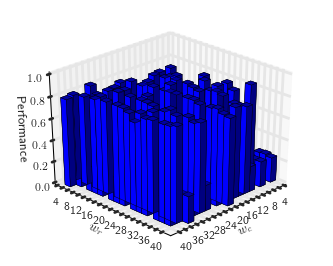
\includegraphics[width=1.0\columnwidth]{img/motivation_1}
      \vspace{-1.5em} % Shrink vertical padding
      \caption{}
      \label{fig:motivation-1}
    \end{subfigure}
    ~%
    \begin{subfigure}[h]{.48\columnwidth}
      \centering
      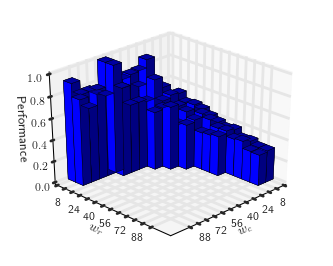
\includegraphics[width=1.0\columnwidth]{img/motivation_2}
      \vspace{-1.5em} % Shrink vertical padding
      \caption{}
      \label{fig:motivation-2}
    \end{subfigure}
    \caption{%
      The performance of different workgroup sizes for the same stencil
      program on two different devices: (\subref{fig:motivation-1})
      Intel CPU, (\subref{fig:motivation-2}) NVIDIA GPU. Selecting an
      appropriate workgroup size depends on the execution device.%
    }
    \label{fig:motivation-arch}
  \end{minipage}%
}%
\hspace{2.5mm}
\adjustbox{valign=t}{%
  \begin{minipage}{.48\textwidth}
    \centering
    \begin{subfigure}[h]{.48\columnwidth}
      \centering
      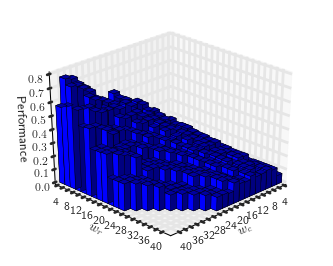
\includegraphics[width=1.0\columnwidth]{img/motivation_3}
      \vspace{-1.5em} % Shrink vertical padding
      \caption{}
      \label{fig:motivation-3}
    \end{subfigure}
    ~%
    \begin{subfigure}[h]{.48\columnwidth}
      \centering
      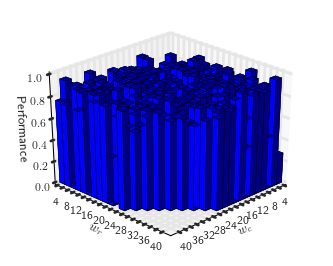
\includegraphics[width=1.0\columnwidth]{img/motivation_4}
      \vspace{-1.5em} % Shrink vertical padding
      \caption{}
      \label{fig:motivation-4}
    \end{subfigure}
    \caption{%
      The performance of different workgroup sizes for the same device
      executing two different stencil programs. Selecting an appropriate
      workgroup size depends on the program.%
    }
    \label{fig:motivation-prog}
  \end{minipage}%
}
\end{figure}

By way of motivating the development of autotuning for Algorithmic Skeletons, we provide a brief examination of the performance impact the OpenCL workgroup size parameter has on the performance of Stencil skeletons in SkelCL (see Section~\ref{sec:omnitune-skelcl} for a full explanation). SkelCL uses OpenCL to parallelise skeleton operations on GPUs and CPUs across many threads~\cite{Steuwer2011}. In OpenCL, multiple threads are grouped into \emph{workgroups}. The shape and size of these workgroups is known to have a big impact on performance. For the SkelCL stencil skeleton, the selection of workgroup size presents a two dimensional parameter space of rows ($w_r$) and columns ($w_c$). Measuring and plotting the runtime of SkelCL stencil kernels using different workgroup sizes allows us to compare the performance of different workgroup sizes for different combinations of architecture and program. Figure~\ref{fig:motivation-arch} shows this performance comparison for a single stencil program on two different devices, demonstrating that a good choice of workgroup size is device dependent. The optimization space of the same stencil kernel on different devices is radically different: not only does the optimal workgroup size change between devices, but the performance of suboptimal workgroup sizes is also dissimilar. The optimization space of~\ref{fig:motivation-1} has a grid-like structure, with clear performance advantages of workgroup sizes at multiples of 8 for $w_c$. A developer specifically targeting this device would learn to select workgroup sizes following this pattern. This domain specific knowledge clearly does not transfer to the device shown in~\ref{fig:motivation-2}.

In Figure~~\ref{fig:motivation-prog}, we compare the performance of two different stencil programs on the \emph{same} device, showing that workgroup size choice is also program dependent. In each of these four examples, the optimal workgroup size changes, as does the relative performance of suboptimal parameters. The average speedup of the best over the worst workgroup size is $37.0\times$, and the average performance that can be achieved using a single fixed workgroup size is only 63\% of the maximum performance achieved using a different workgroup size for each situation.

SkelCL uses a fixed workgroup size by default. Since both the execution device and the user-provided stencil code are not known until runtime, dynamic selection of workgroup size can provide clear performance benefits. To the best of our knowledge, there is currently no such generic system meeting our requirements for lightweight runtime machine learning autotuning with distributed training sets.


\section{The OmniTune Framework}\label{sec:autotune}

\begin{figure}
\centering
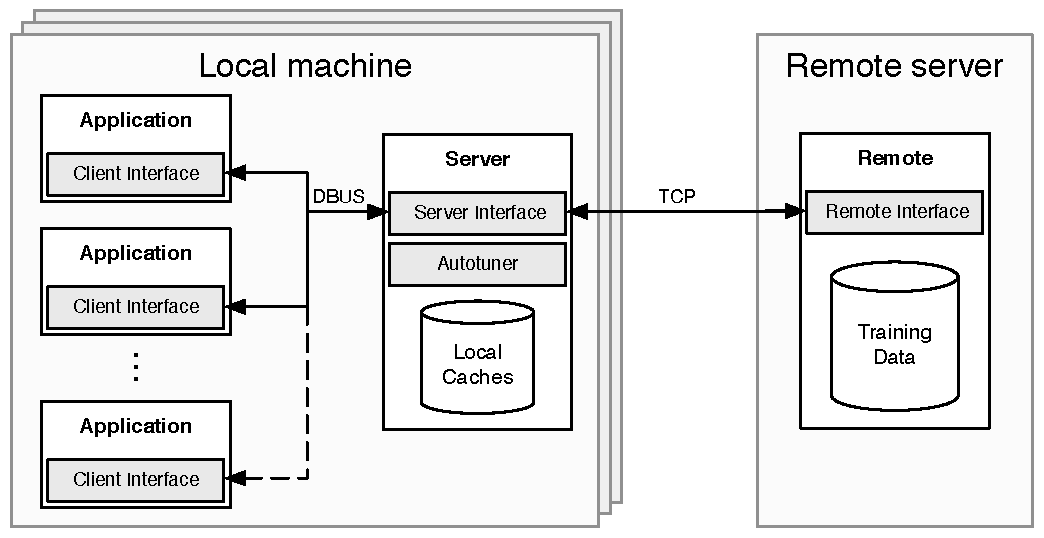
\includegraphics[width=.6\columnwidth]{img/omnitune-system-overview.pdf}
\caption{%
  OmniTune system architecture, showing the separate components and
  the many to one relationship between client applications and
  servers, and servers to remotes.%
  % \vspace{-2em}%
}
\label{fig:omnitune-system-overview}
\end{figure}

OmniTune is our novel open source\footnote{OmniTune source code available
  at: \url{http://chriscummins.cc/s/omnitune}.}, framework for
distributed autotuning of Algorithmic Skeletons using machine
learning. It is an extensible, generic platform for developing
autotuning solutions, aiming to reduce both the engineering effort
required to target new optimization parameters, and the time to
deployment on new systems.

OmniTune emphasizes collaborative learning of optimization spaces. A
client-server architecture with clearly delineated separation of
concerns minimizes the code footprint in client applications, and enables
quick re-purposing for new autotuning targets. OmniTune provides a
lightweight interface for communication between each of the
components, and aims to strike a balance between offering a fully
featured environment for quickly implementing autotuning, while
providing enough flexibility to cater to a wide range of use
cases. First, we describe the overall structure of OmniTune and the
rationale for the design, followed by the interfaces and steps
necessary to integrate OmniTune with a Skeleton library.


\subsection{System Architecture}

OmniTune is built around a three tier client-server architecture,
shown in Figure~\ref{fig:omnitune-system-overview}. The applications
which are to be autotuned are the \emph{clients}. These clients
communicate with a system-wide \emph{server}, which handles autotuning
requests. The server communicates and caches data sourced from a
\emph{remote} server, which maintains a global store of all autotuning
data. There is a many to one relationship between clients, servers,
and remotes, such that a single remote may handle connections to
multiple servers, which in turn may accept connections from multiple
clients. This design has two primary advantages: the first is that it
decouples the autotuning logic from that of the client program,
allowing developers to easily repurpose the autotuning framework to
target additional optimization parameters without a significant
development overhead for the target applications; the second advantage
is that this enables collective tuning, in which training data
gathered from a range of devices can be accessed and added to by any
OmniTune server.

Common implementations of autotuning in the literature either embed
the autotuning logic within each target application
(e.g.~\cite{Chen2014}), or take a standalone approach in which the
autotuner is a separate program which must be externally invoked by
the user (e.g.~\cite{Lutz2013}). Embedding the autotuner within each
target application has the advantage of providing ``always-on''
behavior, but is infeasible for complex systems in which the cost of
building machine learning models must be added to each program
run. The standalone approach separates the autotuning logic, at the
expense of adding one additional step to the build process. The
client-server approach taken in OmniTune aims to combine the
advantages of both techniques by implementing autotuning \emph{as a
  service}, in which a standalone autotuning server performs the heavy
lifting of managing training data and machine learning models, with a
minimal set of lightweight communication logic to be embedded in
target applications.

The OmniTune framework is implemented as a set of Python classes which are extended to target specific parameters. The generic implementation of OmniTune's server and remote components consists of 8987 lines of Python and MySQL code. No predefined client logic is provided, since that is use case dependent (see Section~\ref{sec:omnitune-skelcl} for details of a concrete implementation for SkelCL). Inter-process communication between client programs and the server uses the D-Bus protocol. D-Bus is cross-platform, and bindings are available for most major programming languages, allowing flexibility for use with a range of clients. Communication between servers and remotes uses TCP/IP (we used an Amazon Web Services instance for testing).


\subsection{Autotuning Behavior}

The goal of machine learning enabled autotuning is to build models
from empirical performance data of past programs to select parameter
values for new \emph{unseen} programs. Instead of an iterative search
for good parameters, parameter values are \emph{predicted} based on
models built from measured performance and \emph{features}
(explanatory variables) of past values. The data used to build such
models is called training data. OmniTune supports autotuning using a
separate offline training phase, online training, or a mixture of
both. For each autotuning-capable machine, an OmniTune server hosts
the autotuning logic. On launch, the server requests the latest
training data from the remote, which it uses to build the relevant
models for performing parameter value prediction. If additional
training data is gathered by the server, this can be uploaded and
synchronized with the remote.

While the data types of the autotuning interface are
application-specific (e.g. a binary flag or one or more numeric
values), the general pattern is that a client application will request
parameter values from an OmniTune server by sending it a set of
explanatory variables. The server will then use machine learning
models to form a prediction for the optimal parameter values and
return these. Crucially, there is a mechanism provided for the client
to \emph{refuse} parameter values. This functionality is provided for
cases where the predicted parameter values are in some way invalid and
do not lead to a valid program.

The server contains a library of machine learning tools to perform parameter prediction, interfacing with the popular datamining software suite Weka\footnote{Weka 3 available at:  \url{http://www.cs.waikato.ac.nz/ml/weka/}}. The provided tools include classifiers, regressors, and a selection of meta-learning algorithms.

OmniTune servers may perform additional feature extraction of
explanatory variables supplied by incoming client requests. The reason
for performing feature extraction on the server as opposed to on the
client side is that this allows the results of expensive operations
(for example, analyzing source code of target applications) to be
cached for use across the lifespan of client applications. The
contents of these local caches are periodically and asynchronously
synced with the remote to maintain a global store of lookup tables for
expensive operations.


\subsection{Interfaces}

\begin{figure}
\centering
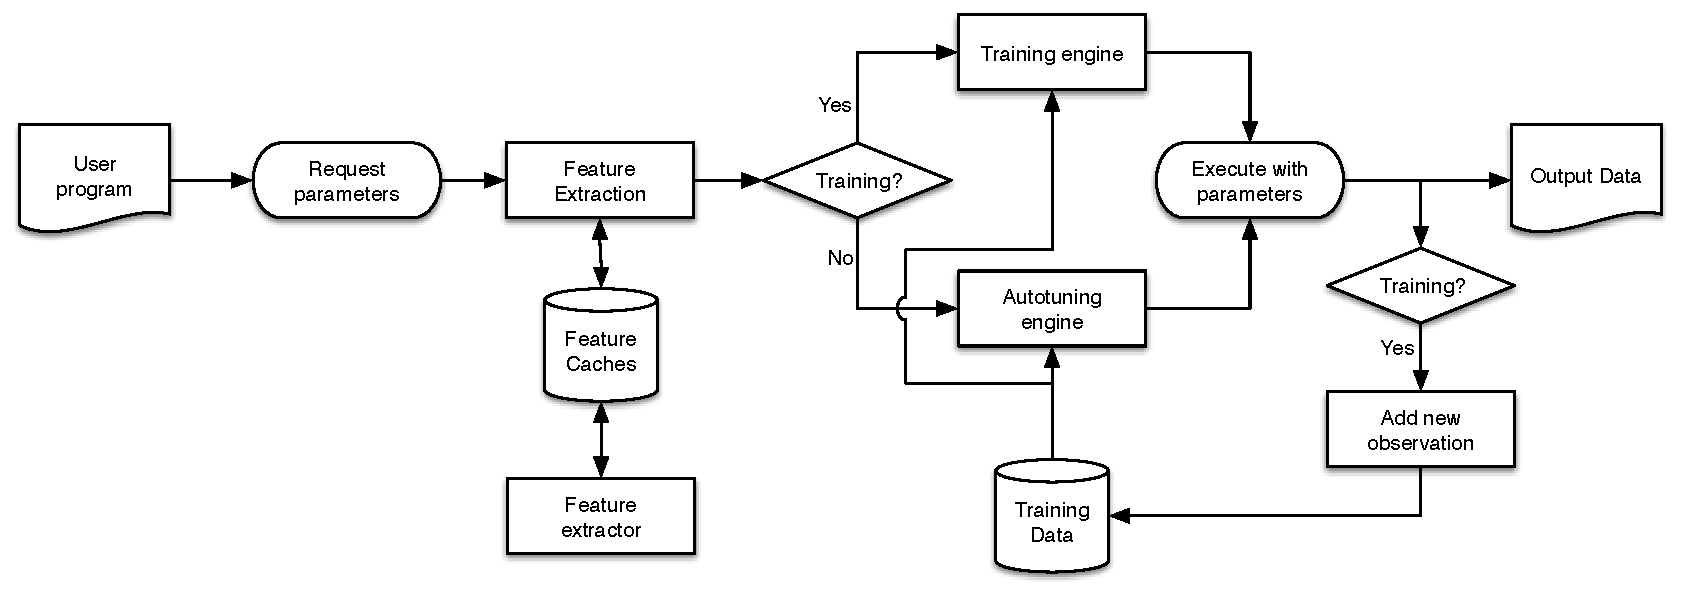
\includegraphics[width=.75\columnwidth]{img/omnitune-system-flow.pdf}
\caption{%
  Predicting parameter values and collecting training data with
  OmniTune.%
}
\label{fig:omnitune-system-flow}
\end{figure}

Key design elements of OmniTune are the interfaces exposed by the
server and remote components.

\paragraph{Client-Server} An OmniTune server exposes a public
interface over D-Bus with four operations. Client applications invoke
these methods to request parameter values, submit new training
observations, and refuse suggested parameters:
%
\begin{itemize}
\item \textsc{Request}$(x) \to p$\\*Given explanatory variables $x$,
  request the parameter values $p$ which are expected to provide
  maximum performance.
\item \textsc{RequestTraining}$(x) \to p$\\*Given explanatory
  variables $x$, allow the server to select parameter values $p$ for
  evaluating their fitness.
\item \textsc{Submit}$(x, p, y)$\\*Submit an observed measurement of
  fitness $y$ for parameter values $p$, given explanatory variables
  $x$.
\item \textsc{Refuse}$(x, p)$\\*Refuse parameter values $p$, given a
  set of explanatory variables $x$. Once refused, those parameters are
  blacklisted and will not be returned by any subsequent calls to
  \textsc{Request()} or \textsc{RequestTraining()} for the same
  explanatory variables $x$.
\end{itemize}
%
% This set of operations enables the core functionality of an
% autotuner, while providing flexibility for the client to control how
% and when training data is collected.

\paragraph{Server-Remote} The role of the remote is to provide
bookkeeping of training data for machine learning. Remotes allow
shared access to data from multiple servers using a transactional
communication pattern, supported by two methods:
%
\begin{itemize}
\item \textsc{Push}$(\bf{x}, \bf{p}, \bf{y})$\\*Asynchronously submit
  training data as three lists: explanatory variables $\bf{x}$,
  parameter values $\bf{p}$, and observed outcomes $\bf{y}$.
\item \textsc{Pull}$() \to (\bf{x}, \bf{p}, \bf{y})$\\*Request
  training data as three lists: explanatory variables $\bf{x}$,
  parameter values $\bf{p}$, and observed outcomes $\bf{y}$.
\end{itemize}


\subsection{Extensibility}

To extend OmniTune to target an optimization parameter, a developer
extends the Python server class to implement response handlers for the four
public interface operations, and then inserts client code into the
target application to call these operations. The implementation of
these response handlers and invoking client code determines the type
of autotuning methods supported. Figure~\ref{fig:omnitune-system-flow}
shows the flow diagram for an example OmniTune implementation. The
call to \textsc{RequestTraining()} is matched with a response call of
\textsc{Submit()}, showing the client recording a training
observation. In the next Section, we will detail the steps required to
apply OmniTune to SkelCL.


\section{Integration of OmniTune with SkelCL}\label{sec:omnitune-skelcl}

In this section we demonstrate the practicality of OmniTune by integrating the framework into an established open source\footnote{SkelCL source code available at:  \url{https://github.com/skelcl/skelcl}} Algorithmic Skeleton library. Introduced in~\cite{Steuwer2011}, SkelCL enables users to easily harness the power of GPUs and CPUs for data parallel computing, offering a set of OpenCL implementations of data parallel skeletons in a C++ library. Skeletons are parameterised with user functions which are compiled into OpenCL kernels for execution on GPUs and CPUs.

\subsection{The Stencil Skeleton}

\begin{figure}
  \centering
  \begin{subfigure}[h]{.55\columnwidth}
    \centering
    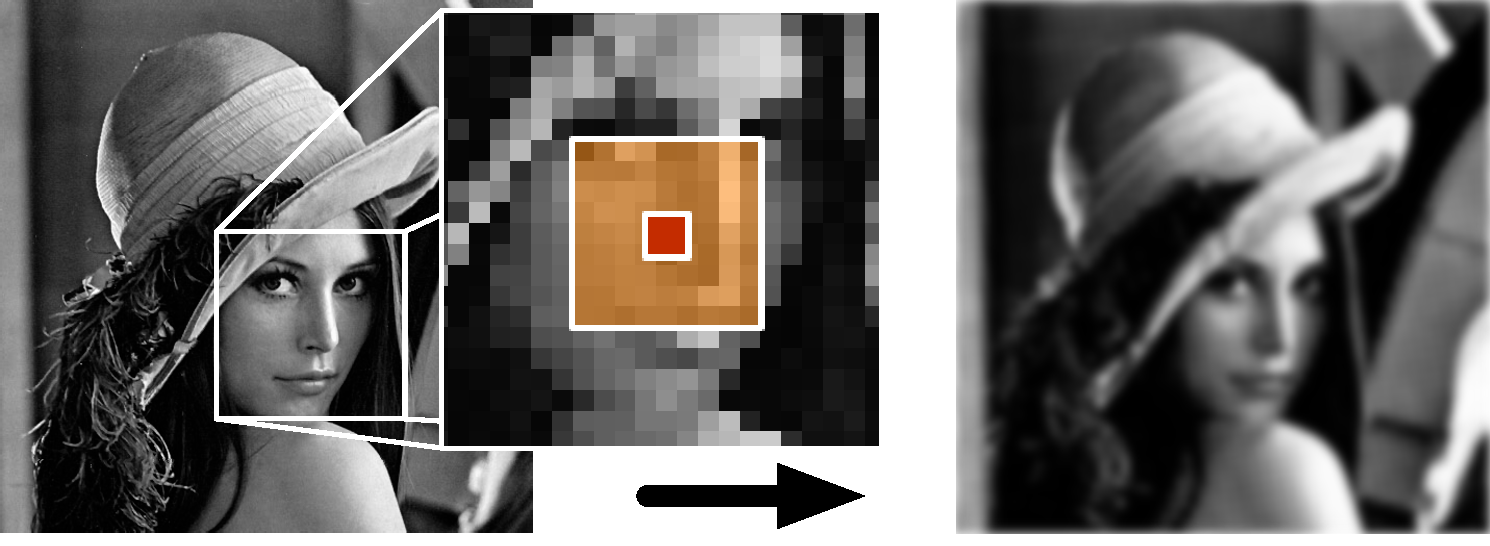
\includegraphics[width=\textwidth]{img/lena-stencil}
  \end{subfigure}
  \begin{subfigure}[h]{.4\columnwidth}
    \centering
    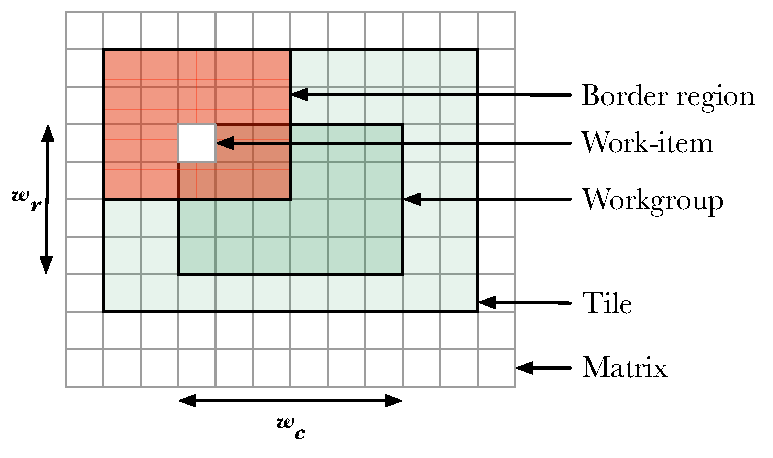
\includegraphics[width=\columnwidth]{stencil}
  \end{subfigure}
  \caption{%
    Application of a Gaussian blur stencil operation to an image: the
    input pixels are decomposed into workgroups, consisting of
    $w_r \times w_c$ elements. Each element is mapped to a
    work-item. Each work-item operates on its corresponding element
    and a surrounding border region. In a Gaussian blur, pixel values
    are interpolated with neighboring pixels, producing a smoothed
    effect.%
  }
  \label{fig:stencil-img}
\end{figure}

Stencils are patterns of computation which operate on uniform grids of
data, where the value of each grid element (cell) is updated based on
its current value and the value of one or more neighboring elements,
called the \emph{border region}. Figure~\ref{fig:stencil-img} shows
the use of a stencil to apply a Gaussian blur to an image. SkelCL
provides a 2D stencil skeleton which allows users to provide a
function which updates a cell's value, while SkelCL orchestrates the
parallel execution of this function across all
cells~\cite{Steuwer2014a}. The border region is described by a
\emph{stencil shape}, which defines an $i \times j$ rectangular region
around each cell which is used to update the cell value. Stencil
shapes may be asymmetrical, and are defined in terms of the number of
cells in the border region to the north, east, south, and west of each
cell $(S_n, S_e, S_s, S_w)$. Given a function $f$, a stencil shape $S$, and an $n \times m$
matrix with elements $x_{ij}$:
%
\begin{equation}
\scriptsize
% \begin{split}
\stencil \left( f, S,
\begin{bmatrix}
  x_{11} & \cdots & x_{1m} \\
  \vdots & \ddots & \vdots \\
  x_{n1} & \cdots & x_{nm}
\end{bmatrix} \right)
\to
\begin{bmatrix}
  z_{11} & \cdots & z_{1m} \\
  \vdots & \ddots & \vdots \\
  z_{n1} & \cdots & z_{nm}
\end{bmatrix}
% \end{split}
\end{equation}
%
where:
%
\begin{equation}
\scriptsize
z_{ij} = f \left(
\begin{bmatrix}
  x_{i-S_n,j-S_w} & \cdots & x_{i-S_n,j+S_e} \\
  \vdots & \ddots & \vdots \\
  x_{i+S_s,j-S_w} & \cdots & x_{i+S_s,j+S_e}
\end{bmatrix} \right)
\end{equation}
%
For border region elements outside the bounds of the matrix, values
are substituted from either a predefined padding value, or the value
of the nearest element within the matrix, depending on user
preference. A popular usage of Stencil codes is for iterative problem
solving, whereby a stencil operation is repeated over a range of
discrete time steps $0 \le t \le t_{max}$, and $t \in \mathbb{N}$. An
iterative stencil operation $g$ accepts a customizing function $f$, a
Stencil shape $S$, and a matrix $M$ with initial values
$M_{init}$. The value of an iterative stencil can be defined
recursively as:
%
\begin{equation}
\scriptsize
g(f, S, M, t) =
\begin{cases}
  \stencil \left( f, S, g(f, S, M, t-1) \right),& \text{if } t \geq 1\\
  M_{init}, & \text{otherwise}
\end{cases}
\end{equation}
%
Examples of iterative stencils include cellular automata and partial
differential equation solvers.

In the implementation of the SkelCL stencil skeleton, each element in
the matrix is mapped to a unique thread (known as a \emph{work item}
in OpenCL) which applies the user-specified function. The work items
are then divided into \emph{workgroups} for execution on the target
hardware. Each work-item reads the value of its corresponding matrix
element and the surrounding elements defined by the border
region. Since the border regions of neighboring elements overlap, the
value of all elements within a workgroup are copied into a
\emph{tile}, allocated as a contiguous region of the fast, but small
local memory. As local memory access times are much faster than that
of global device memory, this greatly reduces the latency of the
border region memory accesses performed by each work item. Changing
the size of workgroups thus directly affects the amount of local memory
required for each workgroup, and in turn affects the number of
workgroups which may be simultaneously active on the device. While the
user defines the data size and type, the shape of the border region,
and the function being applied to each element, it is the
responsibility of the SkelCL stencil implementation to select an
appropriate workgroup size to use.


\subsection{Optimization Parameters}\label{subsec:op-params}

SkelCL stencil kernels are parameterised by a workgroup size $w$,
which consists of two integer values to denote the number of rows and
columns in a workgroup. The space of optimization parameter values is
subject to hard constraints, and these constraints cannot conveniently
be statically determined. Contributing factors are architectural
limitations, kernel constraints, and parameters which are refused for
other reasons.  Each OpenCL device imposes a maximum workgroup size
which can be statically checked. These are defined by architectural
limitations of how code is mapped to the underlying execution
hardware. Typical values are powers of two, e.g.\ 1024, 4096, 8192. At
runtime, once an OpenCL program has been compiled to a kernel, users
can query the maximum workgroup size supported by that particular
kernel dynamically. This value cannot be obtained statically as
there is no mechanism to determine the maximum workgroup size for a
given source code and device without first compiling it, which in
OpenCL does not occur until runtime.

Factors which affect a kernel's maximum workgroup size include the
number of registers required for a kernel, and the available number of
SIMD execution units for each type of instructions in a kernel. In
addition to satisfying the constraints of the device and kernel, not
all points in the workgroup size optimization space are guaranteed to
provide working programs. A \emph{refused parameter} is a workgroup
size which satisfies the kernel and architectural constraints, yet
causes a \texttt{CL\_OUT\_OF\_RESOURCES} error to be thrown when the
kernel is enqueued. Note that in many OpenCL implementations, this
error type acts as a generic placeholder and may not necessarily
indicate that the underlying cause of the error was due to finite
resources constraints. We define a \emph{legal} workgroup size as one
which, for a given \emph{scenario} $s$ (a combination of program,
device, and dataset), satisfies the architectural and kernel
constraints, and is not refused. The subset of all possible workgroup
sizes $W_{legal}(s) \subset W$ that are legal for a given scenario $s$
is then:
%
\begin{equation}
  W_{legal}(s) = \left\{w | w \in W, w < W_{\max}(s) \right\} - W_{refused}(s)
\end{equation}
%
Where $W_{\max}(s)$ can be determined at runtime prior to the kernels
execution, but the set $W_{refused}(s)$ can only be determined
experimentally.

The \emph{oracle} workgroup size $\Omega(s) \in W_{legal}(s)$ of a scenario $s$ is the $w$ value which provides the lowest mean runtime. The relative performance $p(s,w)$ of a particular workgroup size against the maximum available performance for that scenario, within the range $0 \le p(s,w) \le 1$, is the ratio of the runtime of a program with workgroup size $w$ over the oracle workgroup size $\Omega(s)$. For a given workgroup size, the average performance $\bar{p}(w)$ across a set of scenarios $S$ can be found using the geometric mean of performance relative to the oracle:
%
\begin{equation}
  \bar{p}(w) =
  \left(
    \prod_{s \in S} p(s, w)
  \right)^{1/|S|}
\end{equation}
%
The \emph{baseline} workgroup size $\bar{w}$ is the value which
provides the best average case performance across a set of
scenarios. Such a baseline value represents the \emph{best} possible
performance which can be achieved using a single, statically chosen
workgroup size. By defining $W_{safe} \in W$ as the intersection of
legal workgroup sizes, the baseline can be found using:
%
\begin{align}
W_{safe} &= \cap \left\{ W_{legal}(s) | s \in S \right\}\\
\bar{w} &= \argmax_{w \in W_{safe}} \bar{p}(w)
\end{align}


\subsection{Machine Learning}

This section presents three contrasting methods for predicting
workgroup sizes of \emph{unseen} scenarios.


\subsubsection{Predicting Oracle Workgroup Sizes}

\begin{algorithm}[t]
  \SetAlgoLined
  \KwData{scenario $s$}
  \KwResult{workgroup size $w$}
  \SetKwRepeat{Do}{do}{while}

  $w \leftarrow \text{classify}(f(s))$\;
  $W \leftarrow \left\{ w | w < W_{\max}(s) \right\} - W_{refused}(s)$\;
  \While{$w \not\in W_{legal}(s)$}{%
    $W = W - \{w\}$\;
    \eIf{random}{%
      $w \leftarrow $ random selection $w \in W$\;
    }{%
      $d_{min} \leftarrow \infty$; $w_{closest} \leftarrow \text{null}$\;
      \For{$c \in W$}{
        $d \leftarrow \sqrt{\left(c_r - w_r\right)^2 + \left(c_c - w_c\right)^2}$\;
        \If{$d < d_{min}$}{%
          $d_{min} \leftarrow d$\;
          $w_{closest} \leftarrow c$\;
        }
      }
      $w \leftarrow w_{closest}$\;
    }
  }
\caption{Prediction using classifiers}
\label{alg:autotune-classification}
\end{algorithm}

The first approach is detailed in
Algorithm~\ref{alg:autotune-classification}. By considering the set of
possible workgroup sizes as a hypothesis space, we train a classifier
to predict, for a given set of features, the \emph{oracle} workgroup
size. The oracle workgroup size $\Omega(s)$ is the workgroup size
which provides the lowest mean runtime $t(s,w)$ for a scenario $s$:
%
\begin{equation}
  \Omega(s) = \argmin_{w \in W_{legal}(s)} t(s,w)
\end{equation}
%
Training a classifier for this purpose requires pairs of stencil
features $f(s)$ to be labeled with their oracle workgroup size for a
set of training scenarios $S_{training}$:
%
\begin{equation}
  D_{training} = \left\{ \left(f(s), \Omega(s)\right) | s \in S_{training} \right\}
\end{equation}
%
After training, the classifier predicts workgroup sizes for unseen
scenarios from the set of oracle workgroup sizes from the training
set. This is a common and intuitive approach to autotuning, in that a
classifier predicts the best parameter value based on what worked well
for the training data. However, given the constrained space of
workgroup sizes, this presents the problem that future scenarios may
have different sets of legal workgroup sizes to that of the training
data, i.e.:
%
\begin{equation}
  \bigcup_{\forall s \in S_{future}} W_{legal}(s) \nsubseteq \left\{ \Omega(s) | s \in S_{training} \right\}
\end{equation}
%
This results in an autotuner which may predict workgroup sizes that
are not legal for all scenarios, either because they exceed
$W_{\max}(s)$, or because parameters are refused,
$w \in W_{refused}(s)$. For these cases, we evaluate the effectiveness
of three \emph{fallback strategies}:
%
\begin{enumerate}
\item \emph{Baseline} --- select the workgroup size which provides the
  highest average case performance from the set of safe workgroup sizes.
\item \emph{Random} --- select a random workgroup size which is
  expected from prior observations to be legal.
\item \emph{Nearest Neighbor} --- select the workgroup size which
  from prior observations is expected to be legal, and has the lowest
  Euclidian distance to the prediction.
\end{enumerate}


\subsubsection{Predicting Kernel Runtimes}

\begin{algorithm}[t]
  \SetAlgoLined
  \KwData{scenario $s$, regressor $R(x, w)$, fitness function $\Delta(x)$}
  \KwResult{workgroup size $w$}
  \SetKwRepeat{Do}{do}{while}

  $W \leftarrow \left\{ w | w < W_{\max}(s) \right\} - W_{refused}(s)$\;
  % \Comment Candidates.
  \Do{$w \not\in W_{legal}(s)$}{%
    $w \leftarrow \underset{w \in W}{\argmax} \Delta(R(f(s), w))$\;
    % \Comment Select best candidate.
    $W \leftarrow W - \left\{ w \right\}$\;
    % \Comment Remove candidate from selection.
  }
\caption{Prediction using regressors}
\label{alg:autotune-regression}
\end{algorithm}

A problem of predicting oracle workgroup sizes is that, for each
training instance, an exhaustive search of the optimization space must
be performed in order to find the oracle workgroup size. An
alternative approach is to instead predict the expected \emph{runtime}
of a kernel given a specific workgroup size. Given training data
consisting of $(f(s),w,t)$ tuples, where $f(s)$ are scenario features,
$w$ is the workgroup size, and $t$ is the observed runtime, we train a
regressor $R(f(s), w)$ to predict the runtime of scenario and
workgroup size combinations. The selected workgroup size
$\bar{\Omega}(s)$ is then the workgroup size from a pool of candidates
which minimizes the output of the
regressor. Algorithm~\ref{alg:autotune-regression} formalizes this
approach of autotuning with regressors. A fitness function $\Delta(x)$
computes the reciprocal of the predicted runtime so as to favor
shorter over longer runtimes. Note that the algorithm is self
correcting in the presence of refused parameters --- if a workgroup
size is refused, it is removed from the candidate pool, and the next
best candidate is chosen. This removes the need for fallback
handlers. Importantly, this technique allows for training on data for
which the oracle workgroup size is unknown, and has the secondary
advantage that this allows for an additional training instance to be
gathered every time a kernel is evaluated.


\subsubsection{Predicting Relative Performance}

Accurately predicting the runtime of arbitrary code is a difficult
problem. It may instead be more effective to predict the relative
performance of two different workgroup sizes for the same kernel. To
do this, we predict the \emph{speedup} of a workgroup size over a
baseline. This baseline is the workgroup size which provides the best
average case performance across all scenarios and is known to be
safe. Such a baseline value represents the \emph{best} possible
performance which can be achieved using a single, fixed workgroup
size. As when predicting runtimes, this approach performs
classification using regressors
(Algorithm~\ref{alg:autotune-regression}). We train a regressor
$R(f(s), w)$ to predict the relative performance of workgroup size $w$
over a baseline parameter for scenario $s$. The fitness function
returns output of the regressor, so the selected workgroup size
$\bar{\Omega}(s)$ is the workgroup size from a pool of candidates
which is predicted to provide the best relative performance. This has
the same advantageous properties as predicting runtimes, but by
training using relative performance, we negate the challenges of
predicting dynamic code behavior.


\section{Experimental Setup}

To evaluate the performance of the presented autotuning techniques, an
exhaustive enumeration of the workgroup size optimization space for
429 combinations of architecture, program, and dataset was performed.

Table~\ref{tab:hw} describes the experimental platforms and OpenCL devices used. Each platform was unloaded, frequency governors disabled, and benchmark processes set to the highest scheduling priority. Datasets and programs were stored in an in-memory file system.

In addition to synthetic stencil codes, six stencil benchmarks taken from four reference implementations of standard stencil applications from the fields of image processing, cellular automata, and partial differential equation solvers are used: Canny Edge Detection, Conway's Game of Life, Heat Equation, and Gaussian Blur. For each program, datasets of size $512\times512$, $1024\times1024$, $2048\times2048$, and $4096\times4096$ were used.

All runtimes were recorded with millisecond precision using OpenCL's
Profiling API to record the kernel execution time. The workgroup size
space was enumerated for each combination of $w_r$ and $w_c$ values in
multiples of 2, up to the maximum workgroup size. A minimum of 30
samples were recorded for each scenario and workgroup size.

Program behavior is validated by comparing program output against a
gold standard output collected by executing each of the real-world
benchmarks programs using the baseline workgroup size. The output of
real-world benchmarks with other workgroup sizes is compared to this
gold standard output to test for correct program execution.

Five different classification algorithms are used to predict oracle
workgroup sizes, chosen for their contrasting properties: Naive Bayes,
SMO, Logistic Regression, J48 Decision tree, and Random
Forest~\cite{Han2011}. For regression, a Random Forest with regression
trees is used, chosen because of its efficient handling of large
feature sets compared to linear models~\cite{Breiman1999}. The
autotuning system is implemented in Python as a system daemon. SkelCL
stencil programs request workgroup sizes from this daemon, which
performs feature extraction and classification.

\begin{table}
\tiny
\centering
\begin{tabular}{l R{1.1cm} | l R{1.1cm} r R{1.2cm} R{1.2cm} R{1.2cm}}
\toprule
Host & Host Memory &  OpenCL Device &  Compute units & Frequency & Local Memory & Global Cache & Global Memory \\
\midrule
Intel i5-2430M & 8 GB  & CPU              &              4 &   2400 Hz &        32 KB &       256 KB &       7937 MB \\
Intel i5-4570  & 8 GB  & CPU              &              4 &   3200 Hz &        32 KB &       256 KB &       7901 MB \\
Intel i7-3820  & 8 GB  & CPU              &              8 &   1200 Hz &        32 KB &       256 KB &       7944 MB \\
Intel i7-3820  & 8 GB  & AMD Tahiti 7970  &             32 &   1000 Hz &        32 KB &        16 KB &       2959 MB \\
Intel i7-3820  & 8 GB  & Nvidia GTX 590   &              1 &   1215 Hz &        48 KB &       256 KB &       1536 MB \\
Intel i7-2600K & 16 GB & Nvidia GTX 690   &              8 &   1019 Hz &        48 KB &       128 KB &       2048 MB \\
Intel i7-2600  & 8 GB  & Nvidia GTX TITAN &             14 &    980 Hz &        48 KB &       224 KB &       6144 MB \\
\bottomrule
\end{tabular}
\caption{Specification of experimental platforms and OpenCL devices.}
\label{tab:hw}
\end{table}


\section{Performance Results}\label{sec:evaluation}

This section describes the performance results of enumerating the workgroup size optimization space. The effectiveness of autotuning techniques for exploiting this space are examined in Section~\ref{sec:autotuning}. The experimental results consist of measured runtimes for a set of \emph{test cases}, where a test case $\tau_i$ consists of a scenario, workgroup size pair $\tau_i = (s_i,w_i)$, and is associated with a \emph{sample} of observed runtimes of the program. A total of 269813 test cases were evaluated, which represents an exhaustive enumeration of the workgroup size optimization space for 429 scenarios. For each scenario, runtimes for an average of 629 (max 7260) unique workgroup sizes were measured. The average sample size for each test case is 83 (min 33, total 16917118).

The workgroup size optimization space is non-linear and complex, as shown in Figure~\ref{fig:oracle-param-space}, which plots the distribution of optimal workgroup sizes. Across the 429 scenarios, there are 135 distinct optimal workgroup sizes (31.5\%). The average speedup of the oracle workgroup size over the worst workgroup size for each scenario is $15.14\times$ (min $1.03\times$, max $207.72\times$).

Of the 8504 unique workgroup sizes tested, 11.4\% were refused in one or more test cases, with an average of 5.5\% test cases leading to refused parameters. There are certain patterns to the refused parameters: for example, workgroup sizes which contain $w_c$ and $w_r$ values which are multiples of eight are less frequently refused, since eight is a common width of SIMD vector operations~\cite{IntelCorporation2012}. However, a refused parameter is an obvious inconvenience to the user, as one would expect that any workgroup size within the specified maximum should generate a working program, if not a performant one.


\begin{figure}
  \centering
  \begin{subfigure}[t]{0.45\textwidth}
    \centering
    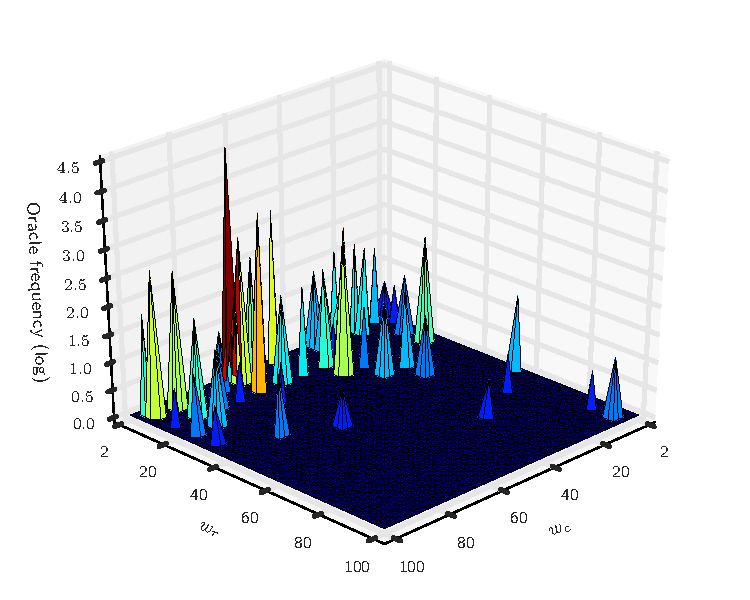
\includegraphics[width=\textwidth]{img/oracle_param_space}
    \vspace{-1.5em} % Shrink vertical padding
    \caption{}
    \label{fig:oracle-param-space}
  \end{subfigure}
  ~%
  \begin{subfigure}[t]{0.45\textwidth}
    \centering
    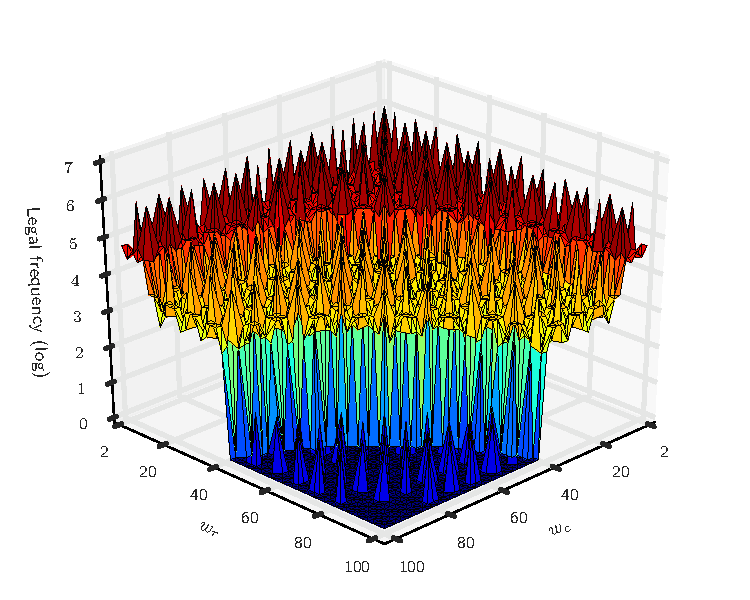
\includegraphics[width=\textwidth]{img/coverage_space}
    \vspace{-1.5em} % Shrink vertical padding
    \caption{}
    \label{fig:coverage}
  \end{subfigure}
  \vspace{-.5em}
  \caption{%
    Log frequency counts for: (\subref{fig:oracle-wgsizes})
    optimality, and (\subref{fig:coverage}) legality for a subset of
    the aggregated workgroup size optimization space,
    $w_c \le 100, w_r \le 100$. The space of oracle workgroup size
    frequencies is highly irregular and uneven, with a most frequently
    optimal workgroup size of $w_{(64 \times 4)}$. Legality
    frequencies are highest for smaller row and column counts (where
    $w < W_{\max}(s) \forall s \in S$), and $w_c$ and $w_r$ values
    which are multiples of 8.%
  }
\label{fig:oracle-wgsizes}
\end{figure}

Experimental results suggest that the problem is vendor --- or at
least device --- specific. Figure~\ref{fig:refused-params} shows the
ratio of refused test cases, grouped by device. We see many more
refused parameters for test cases on Intel CPU devices than any other
type, while no workgroup sizes were refused by the AMD GPU. The exact
underlying cause for these refused parameters is unknown, but can
likely by explained by inconsistencies or errors in specific OpenCL
driver implementations. Note that the ratio of refused parameters
decreases across the three generations of Nvidia GPUs: GTX 590 (2011),
GTX 690 (2012), and GTX TITAN (2013). For now, it is imperative that
any autotuning system is capable of adapting to these refused
parameters by suggesting alternatives when they occur.

\begin{figure}
\centering
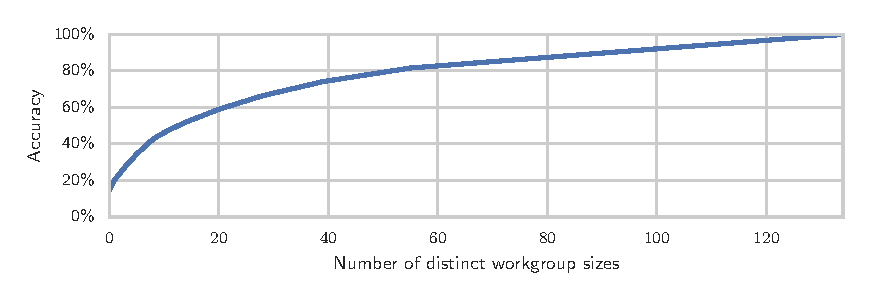
\includegraphics[width=.75\columnwidth]{img/num_params_oracle.pdf}
\caption{%
  Accuracy compared to the oracle as a function of the number of
  unique workgroup sizes. The greatest accuracy that can be achieved
  using a single statically chosen workgroup size is 15\%. Achieving
  50\% oracle accuracy requires a minimum of 14 distinct workgroup
  sizes.%
}
\label{fig:oracle-accuracy}
\end{figure}

The baseline parameter is the workgroup size providing the best
overall performance while being legal for all scenarios. Because of
refused parameters, only a \emph{single} workgroup size
$w_{(4 \times 4)}$ from the set of experimental results is found to
have a legality of 100\%, suggesting that an adaptive approach to
setting workgroup size is necessary not just for the sake of
maximizing performance, but also for guaranteeing program
execution. The utility of the baseline parameter is that it represents
the best performance that can be achieved through static tuning of the
workgroup size parameter; however, compared to the oracle workgroup
size for each scenario, the baseline parameter achieves only 24\% of
the optimal performance.


We find that the \emph{human expert} selected workgroup size is
invalid for 2.6\% of scenarios, as it is refused by 11 test cases. By
device, these are: 3 on the GTX 690, 6 on the i5-2430M, and 2 on the
i5-4570. For the purpose of comparing performance against human
experts, we will ignore these test cases, but it demonstrates the
utility of autotuning not just for maximizing performance, but
ensuring program reliability. For the scenarios where the human expert
workgroup size \emph{is} legal, it achieves an impressive geometric
mean of 79.2\% of the oracle performance. The average speedup of
oracle workgroup sizes over the workgroup size selected by a human
expert is $1.37\times$ (min $1.0\times$, max $5.17\times$).

The utility of the \emph{baseline} workgroup size is that it
represents the best performance that can be achieved through static
tuning. The baseline workgroup size achieves only 24\% of the maximum
performance. Figures~\ref{fig:performance-wgsizes}
and~\ref{fig:performances} show box plots for the performance of all
workgroup sizes using different groupings: ratio of maximum workgroup
size, kernel, device, and dataset. The plots show the median
performance, interquartile range, and outliers. What is evident is
both the large range of workgroup size performances (i.e. the high
performance upper bounds), and the lack of obvious correlations
between any of the groupings and performance.

\begin{figure}
\centering
\adjustbox{valign=t}{%
  \begin{minipage}{.48\textwidth}
    \centering
    \begin{subfigure}[h]{\columnwidth}
      \centering
      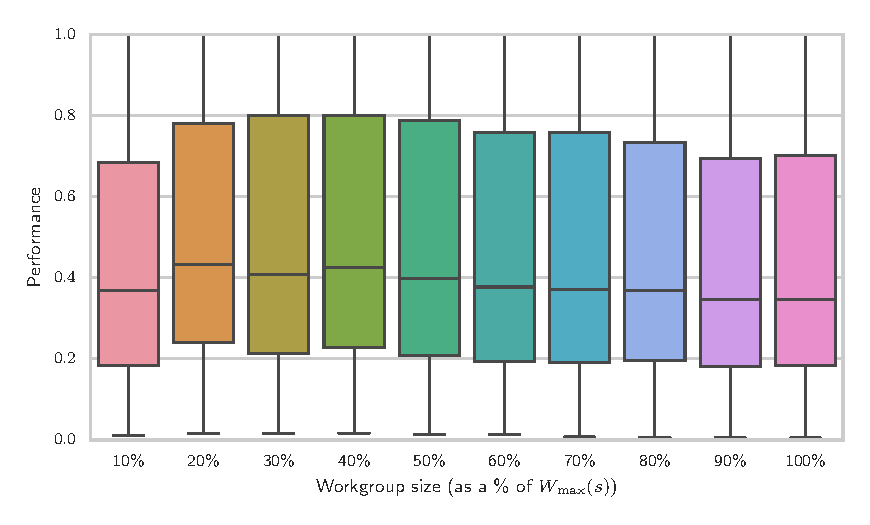
\includegraphics[width=\columnwidth]{img/performance_max_wgsize}
      \vspace{-1.5em} % Shrink vertical padding
      \caption{}
      \label{fig:performance-max-wgsize}
    \end{subfigure}
    \\
    \begin{subfigure}[h]{.48\columnwidth}
      \centering
      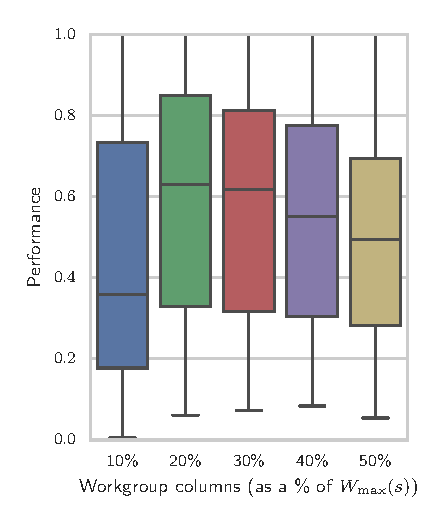
\includegraphics[width=\columnwidth]{img/performance_max_c}
      \vspace{-1.5em} % Shrink vertical padding
      \caption{}
      \label{fig:performance-wg-c}
    \end{subfigure}
    ~%
    \begin{subfigure}[h]{.48\columnwidth}
      \centering
      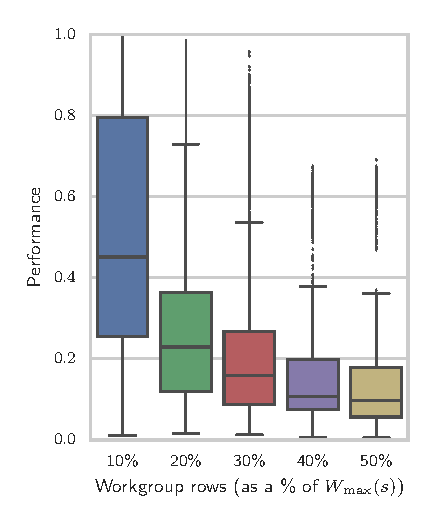
\includegraphics[width=\columnwidth]{img/performance_max_r}
      \vspace{-1.5em} % Shrink vertical padding
      \caption{}
      \label{fig:performance-wg-r}
    \end{subfigure}
    \caption{%
      Comparing performance of workgroup sizes relative to the oracle as
      a function of: (\subref{fig:performance-max-wgsize})~maximum legal
      size, (\subref{fig:performance-wg-c})~number of columns, and
      (\subref{fig:performance-wg-r})~number of rows. Each workgroup
      size is normalized to the maximum allowed for that scenario,
      $W_{\max}(s)$. There is no clear correlation between workgroup
      size and performance.%
    }
    \label{fig:performance-wgsizes}
  \end{minipage}%
}%
\hspace{2.5mm}
\adjustbox{valign=t}{%
  \begin{minipage}{.48\textwidth}
    \centering
    \begin{subfigure}[h]{\columnwidth}
      \centering
      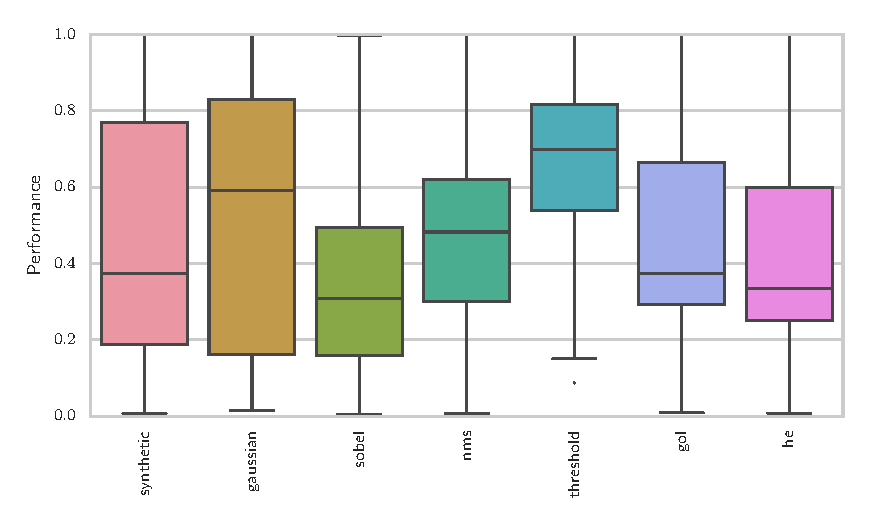
\includegraphics[width=\columnwidth]{img/performance_kernels.pdf}
      \vspace{-1.5em} % Shrink vertical padding
      \caption{}
      \label{fig:performance-kernels}
    \end{subfigure}
    \\
    \begin{subfigure}[h]{.48\columnwidth}
      \centering
      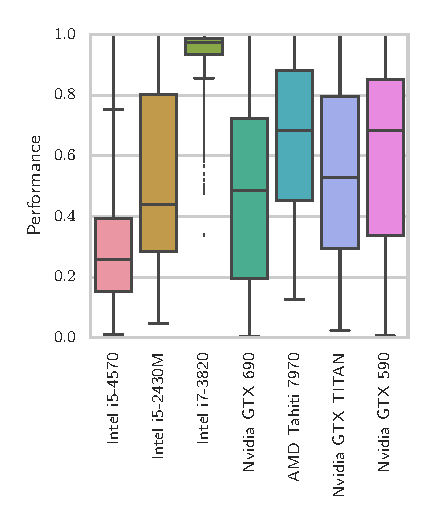
\includegraphics[width=\columnwidth]{img/performance_devices.pdf}
      \vspace{-1.5em} % Shrink vertical padding
      \caption{}
      \label{fig:performance-devices}
    \end{subfigure}
    ~%
    \begin{subfigure}[h]{.48\columnwidth}
      \centering
      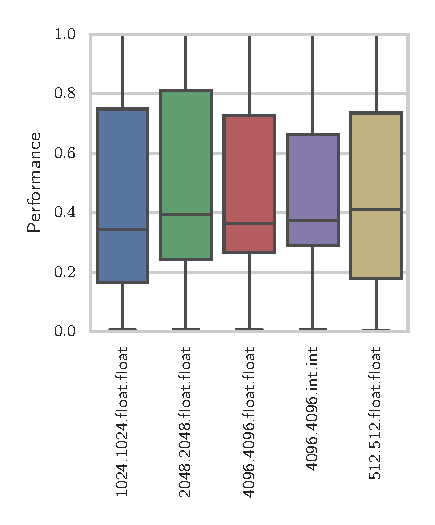
\includegraphics[width=\columnwidth]{img/performance_datasets.pdf}
      \vspace{-1.5em} % Shrink vertical padding
      \caption{}
      \label{fig:performance-datasets}
    \end{subfigure}
    \caption{%
      Performance relative to the oracle of workgroup sizes across all
      test cases, grouped by:
      (\subref{fig:performance-kernels})~kernels,
      (\subref{fig:performance-devices})~devices, and
      (\subref{fig:performance-datasets})~datasets. The performance
      impact is not consistent across kernels, devices, or datasets. The
      Intel i7-3820 has the lowest performance gains from tuning
      workgroup size.%
    }
    \label{fig:performances}
  \end{minipage}%
}
\end{figure}


\begin{figure}
  \centering
  \vspace{-1em}
  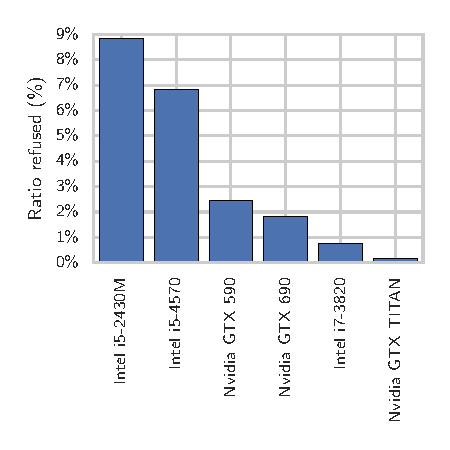
\includegraphics[width=.4\columnwidth]{refused_params_by_device}
  \vspace{-1em}
  \caption{%
    The ratio of test cases with refused workgroup sizes, grouped by
    OpenCL device ID. No parameters were refused by the AMD device.
    \vspace{-1em}%
  }
\label{fig:refused-params}
\end{figure}


\section{Autotuning Evaluation}\label{sec:autotuning}

In this section we evaluate the effectiveness of the three proposed
autotuning techniques for predicting performant workgroup sizes. For
each autotuning technique, we partition the experimental data into
training and testing sets. Three strategies for partitioning the data
are used: the first is a 10-fold cross-validation; the second is to
divide the data such that only data collected from synthetic
benchmarks are used for training and only data collected from the
real-world benchmarks are used for testing; the third strategy is to
create leave-one-out partitions for each unique device, kernel, and
dataset. For each combination of autotuning technique and testing
dataset, we evaluate each of the workgroup sizes predicted for the
testing data using the following metrics:
%
\begin{itemize}
\item time (real) --- the time taken to make the autotuning
  prediction. This includes classification time and any communication
  overheads.
\item accuracy (binary) --- whether the predicted workgroup size is
  the true oracle, $w = \Omega(s)$.
\item validity (binary) --- whether the predicted workgroup size
  satisfies the workgroup size constraints constraints,
  $w < W_{\max}(s)$.
\item refused (binary) --- whether the predicted workgroup size is
  refused, $w \in W_{refused}(s)$.
\item performance (real) --- the performance of the predicted
  workgroup size relative to the oracle for that scenario.
\item speedup (real) --- the relative performance of the predicted
  workgroup size relative to the baseline workgroup size
  $w_{(4 \times 4)}$.
\end{itemize}
%
The \emph{validty} and \emph{refused} metrics measure how often
fallback strategies are required to select a legal workgroup size
$w \in W_{legal}(s)$. This is only required for the classification
approach to autotuning, since the process of selecting workgroup sizes
using regressors respects workgroup size constraints.


\subsection{Predicting Oracle Workgroup Size}

Figure~\ref{fig:class-syn} shows the results when classifiers are
trained using data from synthetic benchmarks and tested using
real-world benchmarks. With the exception of the ZeroR, a dummy
classifier which ``predicts'' only the baseline workgroup size
$w_{\left( 4 \times 4 \right)}$, the other classifiers achieve good
speedups over the baseline, ranging from $4.61\times$ to $5.05\times$
when averaged across all test sets. The differences in speedups
between classifiers is not significant, with the exception of
SimpleLogistic, which performs poorly when trained with synthetic
benchmarks and tested against real-world programs. This suggests the
model over-fitting to features of the synthetic benchmarks which are
not shared by the real-world tests. Of the three fallback handlers,
\textsc{NearestNeighbour} provides the best performance, indicating
that it successfully exploits structure in the optimization space.


\subsection{Predicting with Regressors}

Figure~\ref{fig:regression-class} shows a summary of results for
autotuning using regressors to predict kernel runtimes
(\ref{fig:runtime-class-xval}) and speedups
(\ref{fig:speedup-class-xval}). Of the two regression techniques,
predicting the \emph{speedup} of workgroup sizes is much more
successful than predicting the \emph{runtime}. This is most likely
caused by the inherent difficulty in predicting the runtime of
arbitrary code, where dynamic factors such as flow control and loop
bounds are not captured by the instruction counts which are used as
features for the machine learning models. The average speedup achieved
by predicting runtimes is $4.14\times$. For predicting speedups, the
average is $5.57\times$, the highest of all of the autotuning
techniques.


\subsection{Autotuning Overheads}

Comparing the classification times of Figures~\ref{fig:class-syn}
and~\ref{fig:regression-class} shows that the prediction overhead of
regressors is significantly greater than classifiers. This is because,
while a classifier makes a single prediction, the number of
predictions required of a regressor grows with the size of
$W_{\max}(s)$, since classification with regression requires making
predictions for all $w \in \left\{ w | w < W_{\max}(s) \right\}$. The
fastest classifier is the J48 decision tree, due to the it's
simplicity --- it can be implemented as a sequence of nested
\texttt{if} and \texttt{else} statements. The measured overhead of
autotuning using this classifier is 2.5ms, of which only 0.3ms is
required for classification using Weka, although an optimized decision
tree implementation could reduce this further. The remaining 2.2ms is
required for feature extraction and the inter-process round trip
between the OmniTune server and client.

\begin{figure}
\centering
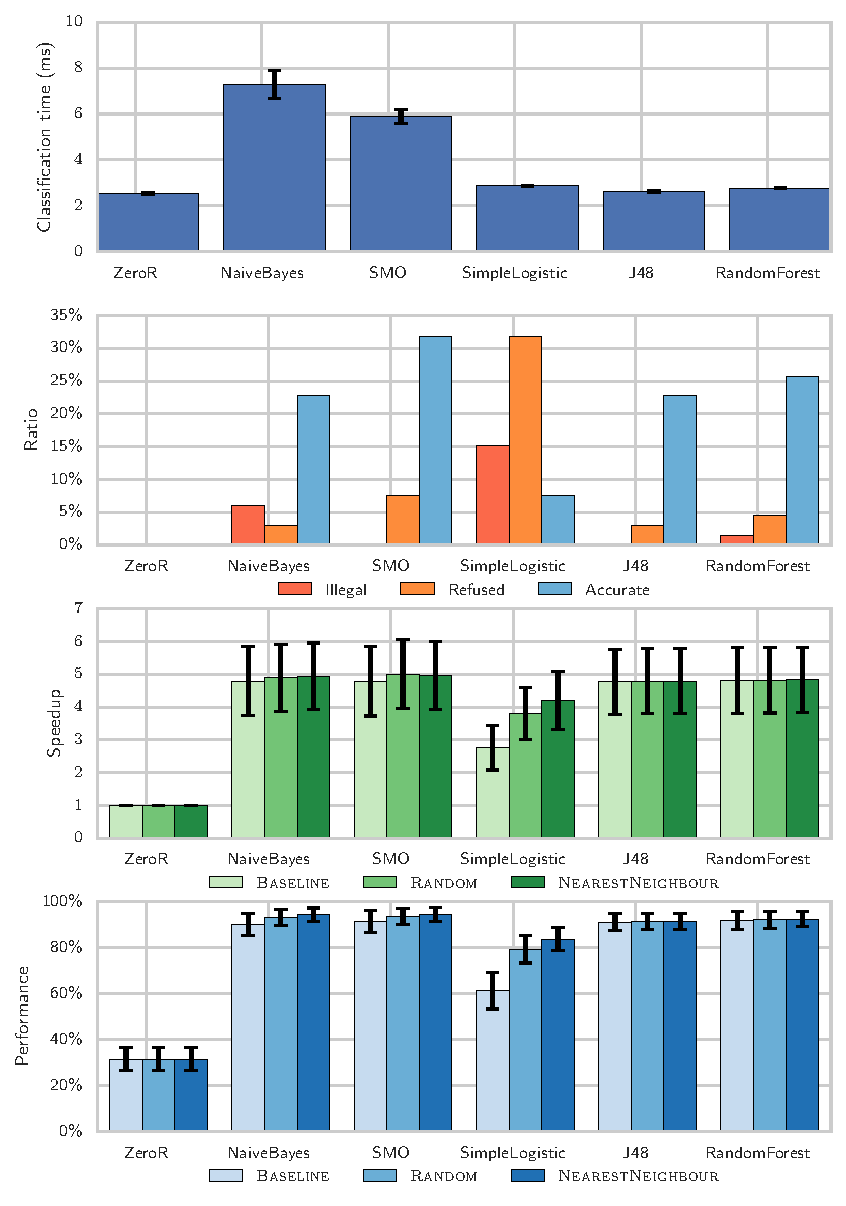
\includegraphics[width=.55\columnwidth]{classification-syn-real}
\vspace{-.7em}
\caption{%
  Autotuning performance using classifiers and synthetic benchmarks. Each
  classifier is trained on data collected from synthetic stencil
  applications, and tested for prediction quality using data from 6
  real-world benchmarks. Each of the different values correspond to a
  different data partitioning strategy, e.g.\ cross-kernel
  partitioning, 10-fold validation, etc. 95\% confidence intervals are
  shown where appropriate.
}
\label{fig:class-syn}
\end{figure}

\begin{figure}
\centering
\begin{subfigure}[h]{.28\columnwidth}
\centering
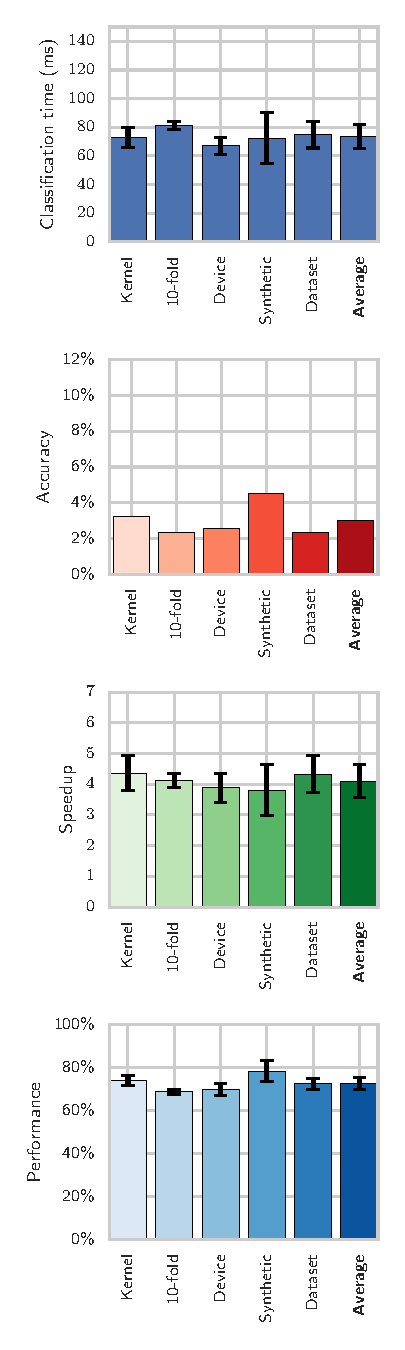
\includegraphics[width=\columnwidth]{runtime-class-xval}
\vspace{-2em}
\caption{}
\label{fig:runtime-class-xval}
\end{subfigure}
\begin{subfigure}[h]{.28\columnwidth}
\centering
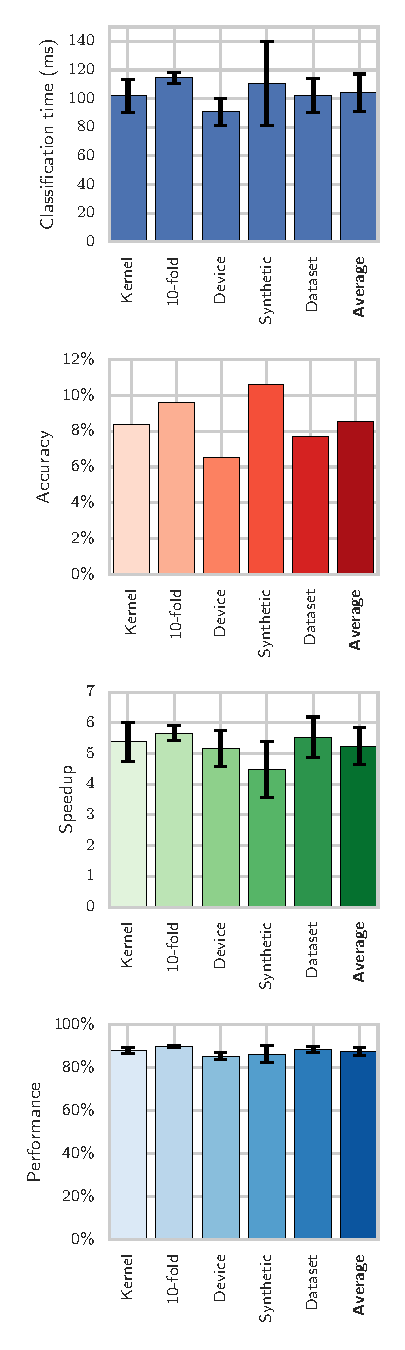
\includegraphics[width=\columnwidth]{speedup-class-xval}
\vspace{-2em}
\caption{}
\label{fig:speedup-class-xval}
\end{subfigure}
\vspace{-.5em}
\caption{%
  Autotuning performance for each type of test dataset using
  regressors to predict: (\subref{fig:runtime-class-xval}) kernel
  runtimes, and (\subref{fig:speedup-class-xval}) relative performance
  of workgroup sizes.%
}
\label{fig:regression-class}
\end{figure}


\subsection{Comparison with Human Expert}

\begin{figure}
\centering
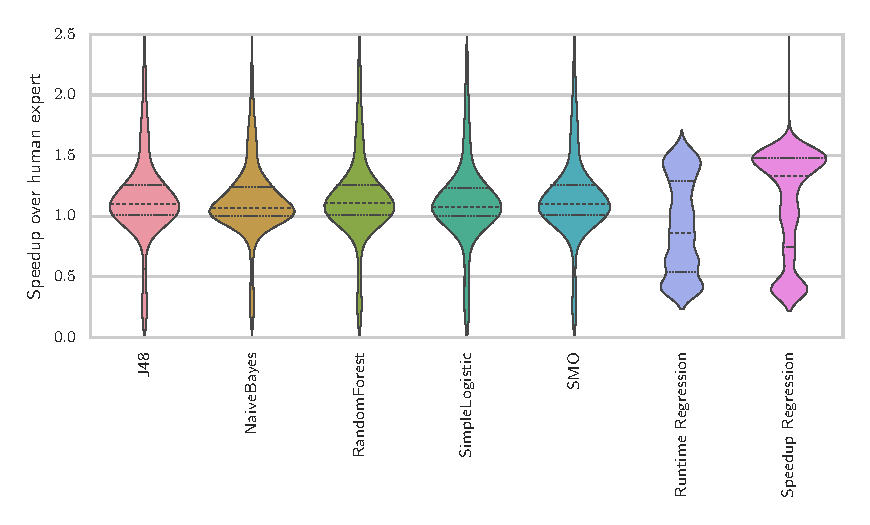
\includegraphics[width=.75\columnwidth]{speedup-distributions}
\vspace{-1.2em}
\caption{%
  Violin plot of speedups over \emph{human expert}, ignoring cases
  where the workgroup size selected by human experts is
  invalid. Classifiers are using \textsc{NearestNeighbour} fallback
  handlers. Horizontal dashed lines show the median, Q1, and
  Q3. Kernel Density Estimates show the distribution of results. The
  speedup axis is fixed to the range 0--2.5 to highlight the IQRs,
  which results in some outlier speedups > 2.5 being clipped.%
}
\label{fig:speedup-distributions}
\end{figure}

In the original implementation of the SkelCL stencil
pattern~\cite{Steuwer2014a}, a workgroup size of $w_{(32 \times 4)}$
was selected in an evaluation of 4 stencil operations on a Tesla S1070
system. In our evaluation of 429 combinations of kernel, architecture,
and dataset, we found that this workgroup size is refused by 2.6\% of
scenarios, making it unsuitable for use as a baseline. However, if we
remove the scenarios for which $w_{(32 \times 4)}$ is \emph{not} a
legal workgroup size, we can directly compare the performance against
the autotuning predictions.

Figure~\ref{fig:speedup-distributions} plots the distributions and
Interquartile Range (IQR) of all speedups over the human expert
parameter for each autotuning technique. The distributions show
consistent classification results for the five classification
techniques, with the speedup at Q1 for all classifiers being
$\ge 1.0\times$. The IQR for all classifiers is $< 0.5$, but there are
outliers with speedups both well below $1.0\times$ and well above
$2.0\times$. In contrast, the speedups achieved using regressors to
predict runtimes have a lower range, but also a lower median and a
larger IQR. Clearly, this approach is the least effective of the
evaluated autotuning techniques. Using regressors to predict relative
performance is more successful, achieving the highest median speedup
of all the techniques of $1.33\times$ over the human expert.


\subsection{OmniTune Extensibility}

The client-server architecture OmniTune neatly separates the
autotuning logic from the target application. This makes adjusting the
autotuning methodology a simple process. To demonstrate this, we
changed the machine learning algorithm from a J48 decision tree to a
Naive Bayes classifier, and duplicated the evaluation. This required
only a single line of source code in the OmniTune server extension to
be changed. Figure~\ref{fig:class-hmaps} visualizes the differences in
autotuning predictions when changing between these two
classifiers. While the average performances of the two classifiers is
comparable, the distribution of predictions is not. For example, the
Naive Bayes classifier predicted the human expert selected workgroup
size of $w_{(32 \times 4)}$ more frequently than it was optimal, while
the decision tree predicted it less frequently. Selection of machine
learning algorithms has a large impact on the effectiveness of
autotuning, and the OmniTune client-server design allows for low cost
experimenting with different approaches. In future work we will
investigate meta-tuning techniques for selecting autotuning
algorithms.

\begin{figure}
\centering
\begin{subfigure}[t]{0.28\columnwidth}
\centering
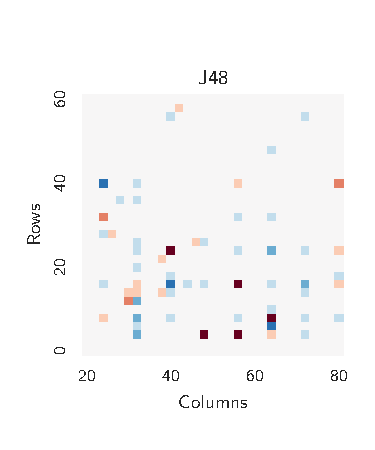
\includegraphics[width=\columnwidth]{img/heatmap_1}
\vspace{-1.5em} % Shrink vertical padding
\caption{}
\label{fig:class-hmaps-1}
\end{subfigure}
~%
\begin{subfigure}[t]{0.28\columnwidth}
\centering
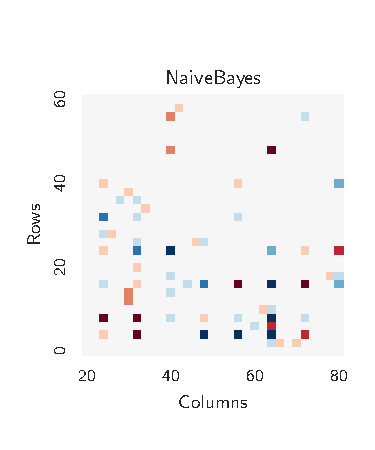
\includegraphics[width=\columnwidth]{img/heatmap_2}
\vspace{-1.5em} % Shrink vertical padding
\caption{}
\label{fig:class-hmaps-2}
\end{subfigure}
~%
\begin{subfigure}[t]{0.28\columnwidth}
\centering
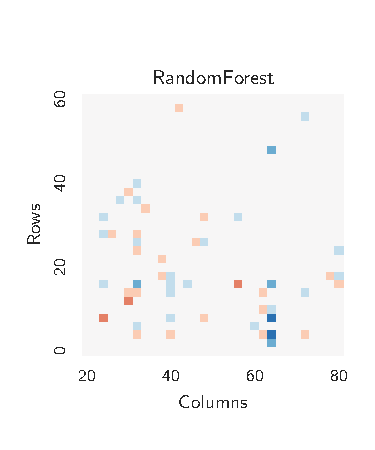
\includegraphics[width=\columnwidth]{img/heatmap_3}
\vspace{-1.5em} % Shrink vertical padding
\caption{}
\label{fig:class-hmaps-3}
\end{subfigure}
\\
\begin{subfigure}[t]{0.28\columnwidth}
\centering
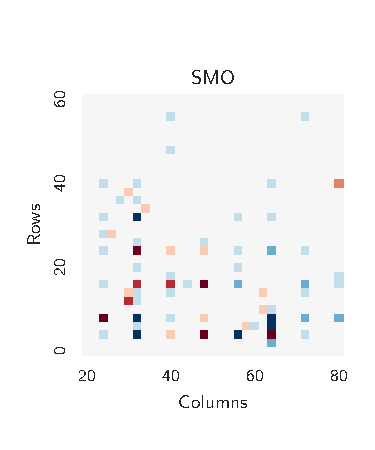
\includegraphics[width=\columnwidth]{img/heatmap_5}
\vspace{-1.5em} % Shrink vertical padding
\caption{}
\label{fig:class-hmaps-4}
\end{subfigure}
~%
\begin{subfigure}[t]{0.28\columnwidth}
\centering
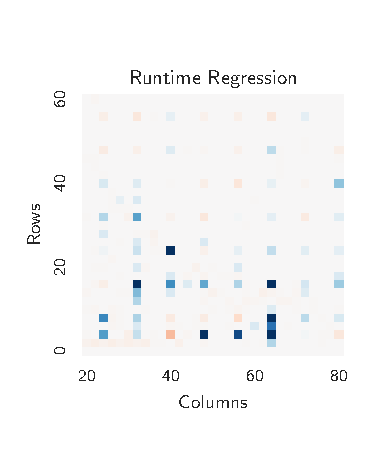
\includegraphics[width=\columnwidth]{img/reg_runtime_heatmap}
\vspace{-1.5em} % Shrink vertical padding
\caption{}
\label{fig:class-hmaps-5}
\end{subfigure}
~%
\begin{subfigure}[t]{0.28\columnwidth}
\centering
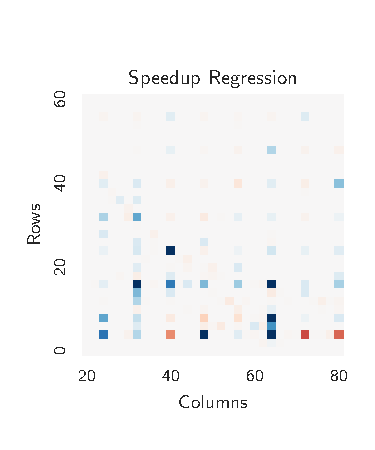
\includegraphics[width=\columnwidth]{img/reg_speedup_heatmap}
\vspace{-1.5em} % Shrink vertical padding
\caption{}
\label{fig:class-hmaps-6}
\end{subfigure}
\caption[Classification error heatmaps]{%
  Heatmaps of classification errors for 10-fold cross-validation,
  showing a subset of the optimization space. The shading in each
  cells indicates if it is predicted less frequently (blue), ore more
  frequently (red) than it is optimal. Color gradients are normalized
  across plots.%
}
\label{fig:class-hmaps}
\end{figure}


\subsection{Summary}

In this section we have explored the performance impact of the
workgroup size optimization space, and the effectiveness of autotuning
using OmniTune to exploit this. By comparing the relative performance
of an average of 629 workgroup sizes for each of 429 scenarios, the
following conclusions can be drawn:

%
\begin{itemize}
\item The performance gap between the best and workgroup sizes for a
  particular combination of hardware, software, and dataset is up to
  $207.72\times$.
\item Not all workgroup sizes are legal, and the space of legal
  workgroup sizes cannot statically be determined. Adaptive tuning is
  required to ensure reliable performance.
\item Statically tuning workgroup size fails to extract the potential
  performance across a range of programs, architectures, and
  datasets. The best statically chosen workgroup size achieves only
  26\% of the optimal performance.
\item Workgroup size prediction using a decision tree achieves an
  average 90\% of the optimal performance.
\item Autotuning provides performance portability across programs,
  devices, and datasets. The performance of predicted workgroup sizes
  for unseen devices is within 8\% of the performance for known
  devices.
\end{itemize}


\section{Related Work}\label{sec:related}

Early work in autotuning applied iterative search techniques to the
space of compiler optimisations~\cite{Bodin1998,Kisuki}. Since then,
machine learning techniques have been successfully employed to reduce
the cost of iterative
compilation~\cite{Agakov,Stephenson2003,Fursin2011}. However,
optimizing for GPU hardware presents different challenges to that of
CPUs. Zero-overhead thread scheduling, memory bandwidth, and thread
grouping optimisations were applied to CUDA matrix multiplication
in~\cite{Ryoo2008a}, enabling speedups of up to $432\times$. The
importance of proper exploitation of local shared memory and
synchronization costs is explored
in~\cite{Lee2010}. In~\cite{Chen2014}, data locality optimisations are
automated using a description of the hardware and a
memory-placement-agnostic compiler. A machine learning model to
predict optimal thread coarsening factors of OpenCL kernels is
presented in~\cite{Magni2014}, demonstrating speedups between
$1.11\times$ and $1.33\times$.

The autotuning frameworks OpenTuner~\cite{Ansel2013} and CLTune~\cite{Nugteren2015} use iterative search techniques to explore optimization spaces. In OpenTuner, using ensemble search techniques; in CLTune, using simulated annealing or particle swarms. Since OpenTuner and CLTune do not \emph{learn} optimization spaces as OmniTune does, performance data is not shared across devices. This means that the search for good parameter values must be repeated for each new device and program to be autotuned. In contrast, our approach combines machine learning with distributed training sets so that these repeated explorations are avoided. \cite{Fursin2015} advocate a ``big data'' driven approach to compiler optimization, where datasets, benchmarks, and metadata about experimental setups are shared in a global repository. This work is complementary to our own, where we have demonstrated the utility of sharing training data for cross-device autotuning. The design of OmniTune is highly optimised for minimal latency autotuning, requiring us to use the client-server architecture to cache local copies of training data, keeping autotuning latency at 2.5ms.

For autotuning stencil codes, \cite{Ganapathi2009} drew upon the
successes of statistical machine learning techniques in the compiler
community, using Kernel Canonical Correlation Analysis to build
correlations between stencil features and optimization
parameters. Their use of KCCA restricts the scalability of their
system, as the complexity of model building grows exponentially with
the number of features. In~\cite{Garvey2015b}, synthetically generated
OpenCL stencils are autotuned for a single GPU using a random forest
classifier to predict memory loading strategy, followed by a heuristic
and an exhaustive search of additional parameter spaces. They evaluate
their system on a single GPU, cross-device performance.

A code generator and autotuner for 3D Jacobi stencil codes is
presented in~\cite{Zhang2013a}, although their approach requires a
full enumeration of the parameter space for each new program, and has
no cross-program learning. A DSL and CUDA code generator for stencils
is presented in~\cite{Kamil2010}. Unlike the SkelCL stencil pattern,
the generated stencil codes do not exploit fast local device
memory. Autotuning memory transfers for multi-GPU stencils is explored
in~\cite{Lutz2013} using a combination of offline tuning and runtime
parameter search. A comparison of tuning for CPU and GPU architectures
is made in~\cite{Christen2011}, although the authors do not compare
differences between GPUs. \cite{Falch2015} use Neural Networks to
autotune three hand-parameter OpenCL benchmarks. Their approach does
not account for invalid parameter values, which causes their autotuner
to predict invalid configurations for some benchmarks.

The automatic generation of synthetic benchmarks using parameterised
template substitution is presented in~\cite{Chiu2015}. The authors
describe an application of their tool for generating OpenCL stencil
kernels for machine learning, but do not report any performance
results.


\section{Conclusions and Future Work}\label{sec:conclusions}

As the trend towards increasingly programmable heterogeneous
architectures continues, the need for industrial quality, high level
abstractions to manage such parallelism will continue to
grow. Autotuning proves to be a valuable aid for achieving these
goals, provided that the burden of development and collecting
performance data is lifted from the user. The system presented in this
paper aims to solve this issue by providing a generic interface for
implementing machine learning-enabled autotuning.

OmniTune is a novel framework for autotuning which has the benefits of
a fast, ``always-on'' interface for client applications, while being
able to synchronize data with global repositories of knowledge which
are built up across devices. To demonstrate the utility of this
framework, we implemented a frontend for predicting the workgroup size
of OpenCL kernels for SkelCL stencil codes. This optimization space is
complex, non linear, and critical for the performance of stencil
kernels.  Selecting the correct workgroup size is difficult ---
requiring a knowledge of the kernel, dataset, and underlying
architecture. The autotuning techniques proposed in this paper achieve
up to 94\% of the maximum performance, providing median speedups of
$3.79\times$ over static tuning and $1.33\times$ over a human expert, while providing robust fallbacks in the presence of unexpected behavior of OpenCL driver implementations.

Of the three techniques proposed, predicting the relative performances
of workgroup sizes using regressors provides the greatest performance
improvements, whilst predicting the oracle workgroup size using
decision tree classifiers adds the lowest runtime overhead. This
presents a trade-off between classification time and training time
which could be explored in future work using a hybrid technique.

In future work we will further explore the transition towards online
machine learning, developing methods for the parallel exploration of
optimization spaces across multiple devices. This will be combined
with the use of adaptive sampling plans to minimize the number of
observations required to distinguish bad from good parameter values.

% TODO: High level patterns as core language features.
% \cite{%
% Stuart2011,% MapReduce on GPUs
% Sander2012,% AMD Bolt C++
% JaredHoberock2014a% ParallelSTL for C++
% }


% bibliography
\newpage % TODO: remove this page break
\bibliographystyle{ACM-Reference-Format-Journals}
\bibliography{refs}


\end{document}
